\chapter{数列的极限}

\section{数列的极限概念}
在前一章中,我们已经看到任何一个实数都可以用有理
数来左、右夹逼,即对于任何实数$x$我们总可以用逼近法求
得两个有理数列$\{a_n\}$, $\{b_n\}$使得
\[a_1\le a_2\le \cdots \le a_n\le \cdots\le x\le \cdots\le b_n\le \cdots\le b_2\le b_1\]
并且$b_n-a_n$可以小到任意小。

数列中的项$a_n$和$b_n$就是$x$的第$n$次不足近似值和过剩近似
值,它们的误差可以用不等式
\[|x-a_n|<b_n-a_n,\qquad |x-b_n|<b_n-a_n\]
来估计。这里所说的逼近的要点在于\textbf{误差可以小到任意小},
下面用例子从另一个角度来说明这一点。

今以$\frac{2}{3}$为例,作上述分析:
\begin{enumerate}
    \item 以3去除2,得:
    \begin{center}
  \longdivision[2]{2.00}{3}      
    \end{center}
    因为每次20除以3都余2, 所以商数6重复出现,这个
    除法可以无止境地作下去。
    \item 上述除式的意义是
\[\begin{split}
    2&=0.6\x3+0.2\Longleftrightarrow 0.6<
\frac{2}{3}<0.7,\\
&=0.66\x3+0.02\Longleftrightarrow 0.66<
\frac{2}{3}<0.67,\\
&=0.666\x3+0.002\Longleftrightarrow 0.666<
\frac{2}{3}<0.667,\\
\cdots &\cdots\cdots\cdots\cdots\cdots\cdots\cdots
\end{split}\]
\end{enumerate}

从上面的分析,同学们可以看出$\frac{2}{3}$
显然不能用有限位
小数表示出,但是存在着由有限位小数所成的无穷数列$\{a_n\}$
和$\{b_n\}$
\[\begin{split}
    \{a_n\}&:\quad a_1=0.6,\; a_2=0.66,\; a_3=0.666,\; \ldots ,\; a_n=0.\underbrace{66\cdots66}_{\text{$n$位小数}},\; \ldots\\
    \{b_n\}&:\quad b_1=0.7,\; b_2=0.67,\; b_3=0.667,\; \ldots ,\; b_n=0.\underbrace{66\cdots67}_{\text{$n$位小数}},\; \ldots
\end{split}\]
满足 
\[a_n=0.\underbrace{66\cdots66}_{\text{$n$位小数}}<\frac{2}{3}<0.\underbrace{66\cdots67}_{\text{$n$位小数}}=a_n+\frac{1}{10^n}\]
并且$a_n$与$\frac{2}{3}$
之间的误差
$\left|a_n-\frac{2}{3}\right|<b_n-a_n=\frac{1}{10^n}$, 同样
$b_n$与$\frac{2}{3}$之间误差$\left|b_n-\frac{2}{3}\right|<\frac{1}{10^n}$,只要$n$充分大,误差
可以小到任意小。上面的逼近过程,表明无穷数列$\{a_n\}$, $\{b_n\}$从左、右两方面趋近$\frac{2}{3}$,可以使其误差任意小,$\frac{2}{3}$就是数列$\{a_n\}$的极限,也是数列$\{b_n\}$的极限,用符号表示就是
\[\lim_{n\to\infty}a_n=\frac{2}{3},\qquad \lim_{n\to\infty}b_n=\frac{2}{3}\]
或者用
\[a_n\to \frac{2}{3},\qquad b_n\to\frac{2}{3},\qquad a_n\to \frac{2}{3}\leftarrow b_n\]
来生动地表述上述事实。

从这里我们看到逼近与极限是密切相关的,极限只是把
逼近过程推进到无穷$(n\to\infty)$的结果,逼近只要误差小到
所要求的精确度后就可以停止。$\Lim_{n\to\infty}a_n=\frac{2}{3}$
表示数列$\{a_n\}$当
$n$无限增大的极限值是$\frac{2}{3}$。

我们再用极限的观点对$\sqrt{2}$ 进行分析如下。$\sqrt{2}$是一
个什么数?要回答这个问题,我们只须找出有理数
$\frac{a}{b}$
在什么时候大于$\sqrt{2}$, 什么时候小于$\sqrt{2}$, 也就是说,如果
$\left(\frac{a}{b}\right)^2<2$, 那么正数$\frac{a}{b}<\sqrt{2}$;如果$\left(\frac{a}{b}\right)^2>2$, 那么
$\frac{a}{b}>\sqrt{2}$. 根据有理数是有序的,稠密的,因此有理数的
平方总能和2比较大小,这就保证我们可以用逼近法(譬如
十分逼近法)决定左、右夹逼$\sqrt{2}$的两个由十进位小数组
成的数列$\{a_n\}$、$\{b_n\}$如下:
\[\begin{split}
    \{a_n\}&:\quad a_1=1,\; a_2=1.4,\; a_3=1.41,\; a_4=1.414,\ldots\\
    \{b_n\}&:\quad b_1=2,\; b_2=1.5,\; b_3=1.42,\; b_4=1.415,\ldots\\
\end{split}\]
使得$a_n<\sqrt{2}<b_n$, 而且$b_n-a_n=\frac{1}{10^n}$,
于是
\[|a_n-\sqrt{2}|<\frac{1}{10^n},\qquad |b_n-\sqrt{2}|<\frac{1}{10^n} \]
这就是说,第$n$次的有限小数近似值$a_n$和$b_n$与$\sqrt{2}$的误
差分别小于$\frac{1}{10^n}$,
因此,只要$n$充分大,误差就可以小到任
意小,当我们让这个计算过程,无穷地进行下去时,我们就
说$\sqrt{2}$ 是数列$\{a_n\}$或$\{b_n\}$的极限,记做
\[\lim_{n\to\infty}a_n=\sqrt{2},\qquad \lim_{n\to\infty}b_n=\sqrt{2}\]

从上面两个例子看到,实数是具有$n$位数字的普通十进
位小数数列,当$n$无限增大时的极限。

如今我们说明了逼近与极限概念密切相关的一面,但是
极限与逼近也有观点不同,概念层次也不同的方面,上面所
说用十分逼近法求$\sqrt{2}$ 的近似值$1,1.4,1.41,\ldots$等是逼
近的观点,它是先有$\sqrt{2}$ ,即我们先知道$\sqrt{2}$  是方程$x^2=2$
的根,然后用小数去逐步逼近。极限的观点恰恰相反,它是
先有一个无穷数列$\{a_n\}$,然后要去看一下,它们是否恰好无
限逼近某一个常数$A$. 假如是这样,就叫$A$是数列$\{a_n\}$的极
限值。

下面介绍几个逼近某一常数的无穷数列的例子。

\begin{example}
    仔细观察数列:
    \[1,\; \frac{1}{2},\;\frac{1}{3},\;\frac{1}{4},\; \ldots,\;\frac{1}{n},\;\ldots\]
我们马上看出
\begin{enumerate}
    \item 上述数列的每一项都是正数。
    \item 上述数列逐项递减:
\[1>\frac{1}{2}>\frac{1}{3}>\cdots>\frac{1}{n}>\frac{1}{n+1}>\cdots>0\]
因而是一个递减有界数列。
\item 当$n$愈来愈大时,$a_n=\frac{1}{n}$
愈来愈接近0, 它们的
误差$|a_n-0|=\frac{1}{n}$, 只要充分大,就可以小到任意小。
\end{enumerate}

对于情形3,我们就说:数列$\left\{\frac{1}{n}\right\}$
趋近于0或收敛到0, 或0是数列$\left\{\frac{1}{n}\right\}$
的极限,并记作$\frac{1}{n}\to 0$
或$\Lim_{n\to\infty}\frac{1}{n}=0$。

现在,让我们再用数轴把上述事实图解说明如下:
\begin{figure}[htp]
    \centering
    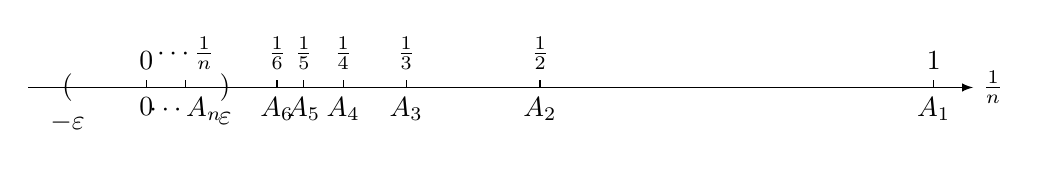
\begin{tikzpicture}[>=latex]
 \draw[->] (-1.5,0)--(10.5,0)node[right]{$\frac{1}{n}$};
\foreach \x/\xtext in {1/A_1,.5/A_2,.33/A_3,.25/A_4,.2/A_5,.166/A_6,0/0}
{
    \draw (\x*10,0)node[below]{$\xtext$}--(\x*10,.1);
}
\foreach \x/\xtext in {1/1,.5/\frac{1}{2},.33/\frac{1}{3},.25/\frac{1}{4},.2/\frac{1}{5},.166/\frac{1}{6},0/0}
{
    \node at (\x*10,.1)[above]{$\xtext$};
}
\node at (-1,0){(};
\node at (1,0){)};
\node at (-1,-.2)[below]{$-\varepsilon$};
\node at (1,-.2)[below]{$\varepsilon$};
\draw (.5,0)node[below]{$\cdots A_n$}--(.5,.1)node[above]{$\cdots \frac{1}{n}$};
    \end{tikzpicture}
    \caption{}
\end{figure}

在数轴上取以数列:
\[1,\; \frac{1}{2},\;\frac{1}{3},\;\frac{1}{4},\; \ldots,\;\frac{1}{n},\;\ldots\]
的各项为坐标的各点,就得到一个点列:
\[A_1,A_2,A_3,A_4,\ldots,A_n,\ldots,\]
上述点列$\{A_n\}$从原点$O$的右边逐步向原点逼近,而且点$A_n$到
原点的距离$|a_n-0|=\frac{1}{n}$,
只要$n$充分大,就可以小到任
意小。上面的事实也可以这样来说明:通常我们把$A$点为中
心的\textbf{开区间}$(A-\varepsilon,A+\varepsilon)$叫做这\textbf{点$A$的$\varepsilon$邻域}。我们看到,
原点$O$的任意$\varepsilon$邻域,包
含$\left\{\frac{1}{n}\right\}$
的除有限个点以外的全部
点。这也就是说数列$\left\{\frac{1}{n}\right\}$
是收敛的,并且收敛到0。
\end{example}

\begin{example}
观察数列$\left\{\frac{n}{n+1}\right\}: \frac{1}{2},\frac{2}{3},\ldots,\frac{n}{n+1},\ldots$
同学们容易看出,这个数列逐项递增,其各项$a_n=\frac{n}{n+1}$
永
远小于1, $a_n$和1之间的误差$|a_n-1|=\left|\frac{-1}{n+1}\right|=\frac{1}{n+1}$,
只要$n$充分大就可以到任意小。这也就是说,这个数列在
数轴上的对应点列,除有限个点外全部点都在点1的 任意$\varepsilon$
邻域内(图3.2),因此,这个数列$\left\{\frac{n}{n+1}\right\}$
的极限是1, 或
者变量$a_n=\frac{n}{n+1}$
的极限是1, 用符号表示就是:
\[\frac{n}{n+1}\to 1,\quad \text{或者}\quad \lim_{n\to\infty}\frac{n}{n+1}=1\]
\begin{figure}[htp]
    \centering
\begin{tikzpicture}[>=latex]
\draw[->] (-.5,0)--(10,0)node[right]{$\frac{n}{n+1}$};
\foreach \x/\xtext in {0/0,.5/\frac{1}{2},.667/\frac{2}{3},.75/\frac{3}{4}, .8/\frac{4}{5},1/1}
{
    \draw (\x*8,0)node[below]{$\xtext$}--(\x*8,.1);
}
\node at (7+.3,0.2)[above]{$1-\varepsilon$};
\node at (9-.3,0.2)[above]{$1+\varepsilon$};
\node at (7+.3,0){(};
\node at (9-.3,0){)};

\end{tikzpicture}  
    \caption{}
\end{figure}
\end{example}

\begin{example}
    观察数列$\left(-\frac{1}{2}\right),\; \left(-\frac{1}{2}\right)^2,\; \left(-\frac{1}{2}\right)^3,\ldots,\left(-\frac{1}{2}\right)^n,\;\ldots$, 这个数列逐项正负相间,是摆动数列,显然,
    各项的绝对值$|a_n|\le\frac{1}{2}$, $n=1,2,3,\ldots$,因此,它又
    是有界的。其第$n$项与数0之间的误差$|a_n-0|=\left(\frac{1}{2}\right)^n$,当$n$充分大时,可以小到任意小。再从数轴上看,其对应点列从
    原点的左、右两侧向原点逼近,而且当$n$充分大时,$a_n$全部
    都在原点的任意$\varepsilon$邻域内(图7.3),因此,这个数列
$\left\{\left(-\frac{1}{2}\right)^n\right\}$的极限是0。
\begin{figure}[htp]
    \centering
 \begin{tikzpicture}[>=latex]
\draw[->] (-5.5,0)--(5.5,0)node[right]{$\left(-\frac{1}{2}\right)^n$};
\foreach \x/\xtext in {0/0,-1/-1,-.5/-\frac{1}{2},.25/\frac{1}{4},1/1}
{
    \draw (\x*5,0)node[below]{$\xtext$}--(\x*5,.1);
}
\foreach \x/\xtext in {0/{},-1/{},-.5/A_1,.25/A_2,1/{}}
{
    \node at (\x*5,.1)[above]{$\xtext$};
}

\foreach \x/\xtext in {-.125/A_3,.0625/A_4}
{
    \draw (\x*5,0)--(\x*5,.1)node[above]{$\xtext$};
}

\foreach \x/\xtext in {-.15/-\varepsilon,.15/\varepsilon}
{
    \node at (\x*5,-.15)[below]{$\xtext$};
}
\node at (-.75,0){(};
\node at (.75,0){)};


 \end{tikzpicture}   
    \caption{}
\end{figure}
\end{example}

从以上三个数列,我们看到它们的共性是在项数$n$无限
增大的过程中,参与在这个过程的变量$a_n=\frac{1}{n}$, $a_n=\frac{n}{n+1}$, 
$a_n=\left(-\frac{1}{2}\right)^n$
所取的值与某一个常数$A$的差的绝对值$|a_n-
A|$(或者说它们之间的绝对误差),只要$n$充分大,就可
以小到任意小。它们在数轴上对应的点列,只要$n$充分大,
除有限个点外全部点都在点$A$的任意$\varepsilon$邻域内。

让我们把只要$n$充分大,误差可以任意小的含义说得更
精确些。为此,再以例7.3说明之,我们来看它的第$n$项与0
的误差:
\[|a_n-0|=\left|\left(-\frac{1}{2}\right)^n-0\right|=\left(\frac{1}{2}\right)^n\]

当$n$为何值时,$\left(\frac{1}{2}\right)^n<0.0001$。解之,得
\[n\lg\left(\frac{1}{2}\right)<-4,\quad \text{即}\quad (-0.3010)n<-4\]
$\therefore\quad n>13.289$

因此,只须$n\ge 14$, 就有
\[|a_n-0|=\left(\frac{1}{2}\right)^n\le \left(\frac{1}{2}\right)^{14}=0.000061<0.0001\]
这也就是说,对于给定的0.0001, 总能找到这样一个项数,
$N=14$, 使得当$n\ge14$时,其误差
\[|a_n-0|=\left(\frac{1}{2}\right)^{14}<0.0001\]

当$n$为何值时,$\left(\frac{1}{2}\right)^n<\frac{1}{10^8}$
只须,
\[n\lg\left(\frac{1}{2}\right)<-8\]
即
\[n>\frac{-8}{-0.3010}=26.578\]
因此,只须$n\ge 27$时,就有
\[\left(\frac{1}{2}\right)^n<\left(\frac{1}{2}\right)^{27}=0.000000007=7\x 10^{-9}<10^{-8}\]

一般地,任给$\varepsilon >0$, 当$n$为何值时,$\left(\frac{1}{2}\right)^n<\varepsilon$。只须
\[n\lg \frac{1}{2}<\lg\varepsilon\] 
即
\[n>\frac{\lg\varepsilon}{-0.3010}\]
由于$\varepsilon$ 是任意小的正数,当$\varepsilon <1$时,$\lg\varepsilon <0$。于是
$\frac{\lg\varepsilon}{-0.3010}$
是正数,因此,我们总能找到这样项数$N=\left(\frac{\lg\varepsilon}{-0.3010}\text{的整数部分}\right)+1$
,使得当$n\ge N$,
\[|a_n-0|=\left(\frac{1}{2}\right)^n<\left(\frac{1}{2}\right)^N<\varepsilon  \]

现在,我们可以给数列$\{a_n\}$的极限是$A$以精确定义
如下:

\begin{blk}{定义}
    任给正数$\varepsilon$, 总可以定出一个正整数$N$, 使得只
要$n\ge N$时,$|a_n-A|<\varepsilon$都成立,我们就说数列$\{a_n\}$的\textbf{极限
是}A, 或者说数列$\{a_n\}$\textbf{收敛到}$A$。
\end{blk}
 
让我们再对上述定义作几点说明:
\begin{enumerate}
\item $\varepsilon$ (读成Epsilon)是希腊字母,相当于英文字母
的$e$, 它是error(误差)的头一个字母,误差任意小的数
量提法就是“小于任给正数$\varepsilon$”。
\item $a_n$是逐步逼近$A$的,要使误差$|a_n-A|$愈小(或者
说够小)那就要让数列的项数$n$变得够大,所以“只要$n\ge
N$时,$|a_n-A|<\varepsilon$ ”的意义也就是:“只要$n$够大,误差$|a_n
-A|$就会小到所要求的那么小!”
\item $\varepsilon$是任给的正数,是变量,但是当误差范围$\varepsilon$一经
给定之后,就为常数,我们对于这个指定的$\varepsilon$检验是否存在
具有上述性质的$N$, 在求$N$的过程中,$\varepsilon$的值不能变动,一般
说来,给的$\varepsilon$愈小,那么求得的$N$愈大。
\item 定义中的当$n\ge N$时,$|a_n-A|<\varepsilon$等价于当$n\ge N$
时,$A-\varepsilon<a_n<A+\varepsilon$或$a_n\in (A-\varepsilon,A+\varepsilon)$, 这就是说,如
果数列$\{a_n\}$收敛于$A$则在点$A$的任何$\varepsilon$邻域内必包含这个数列
的除有限个项以外的一切项。
\end{enumerate}


为了帮助同学熟悉极限定义,我们在下面再举几个例
子,说明$N$的大小和$\varepsilon$之间的关联,并给出证明某数是已
知数列的极限的方法。

\begin{example}
    证明数列$\left\{\frac{n}{n+1}\right\}$
的极限是1。
\end{example}

\begin{solution}
对于任给$\varepsilon>0$,要使
\[\left|\frac{n}{n+1}-1\right|=\frac{1}{n+1}<\varepsilon\]
只须$n+1>\frac{1}{\varepsilon}$,即$n>\frac{1}{\varepsilon}-1$,取$N=\left(\frac{1}{\varepsilon}-1\right)$
的整数部分$+1$,所以当$n\ge N$时,可使
\[\left|\frac{n}{n+1}-1\right|=\frac{1}{n+1}\le \frac{1}{N+1}<\varepsilon\]
    这就是说$\Lim_{n\to\infty}\frac{n}{n+1}=1$。
\end{solution}

\begin{example}
    证明数列:
$1,0,\frac{1}{2},0,\frac{1}{3},0,\ldots,0,\frac{1}{n},0,\ldots$的极
限是0。
\end{example}

\begin{proof}
  这个数列的通项公式可以写成
\[a_n=\begin{cases}
    0,& \text{当$n$为偶数时;}\\
   \frac{2}{n+1},& \text{当$n$为奇数时。}
\end{cases}\]

对于任给$\varepsilon>0$, 因为数列$\{a_n\}$的所有偶数项为0, 所
以从第二项开始以后的所有偶数项都小于给定的$\varepsilon$. 现在须
从奇数项中确定从哪一项开始以后的一切项与0的误差小
于$\varepsilon$. 

令奇数项与0的误差:$\frac{2}{n+1}<\varepsilon$,即
\[n+1>\frac{2}{\varepsilon},\qquad n>\frac{2}{\varepsilon}-1\]  
取$N=\left(\frac{2}{\varepsilon}-1\right)$的整数部分加1,于是,当$n\ge N$,可使$\frac{2}{n+1}<\varepsilon$。所以对于任给$\varepsilon>0$, 从第$N$项开始以后的一切项都能使
$|a_n-0|<\varepsilon$
成立。即$\Lim_{n\to\infty}a_n=0$。
\end{proof}


\begin{example}
    证明数列$\left\{\frac{n^2-1}{n^2+n+1}\right\}$的极限是1。
\end{example}

\begin{proof}
对于任给$\varepsilon>0$, 
要使
\[|a_n-1|=\left|\frac{n^2-1}{n^2+n+1}-1\right|=\left|\frac{-n-2}{n^2+n+1}\right|=\frac{n+2}{n^2+n+1}<\varepsilon\]
看看是否存在这样的$N$, 使得当$n\ge N$时,永远有$|a_n-1|<\varepsilon$,
可是直接从上面的不等式解出$N$是不容易的,但我们
注意到,当$n$充分大时,在分子中起主导作用的是$n$, 而在
分母中起主导作用$n^2$. 如果把分子扩大为$2n\; (n>2)$, 又
把分母缩小为$n^2$, 这样有
\[|a_n-1|=\frac{n+2}{n^2+n+1}<\frac{2n}{n^2}=\frac{2}{n}\]

现在令$|a_n-1|<\frac{2}{n}<\varepsilon$,即$n>\frac{2}{\varepsilon}$,取$N$为$\frac{2}{\varepsilon}$的整数部分加1, 于是,当$n\ge N$时,可使
\[|a_n-1|>\frac{2}{n}<\varepsilon\]
这就是说$\Lim_{n\to\infty}\frac{n^2-1}{n^2+n+1}=1$。
\end{proof}

在上面的证明中,所取得的$N$比实际所需要的要大一
些,这样并不影响我们所要说明的问题:“$N$是根据预先给
定的$\varepsilon$来确定的,而且这个$N$满足极限定义中的条件”,事
实上,$N$不是由$\varepsilon$唯一确定的,对于给定的$\varepsilon>0$, 如果某
数,譬如10000可以充当极限定义中的$N$, 则大于10000的任
何一个自然数也都可以充当$N$, 自然$N$愈小愈好,但是,有时
候为了便于证明,不妨把$N$取得大些。问题的关键是是否存在
这样的$N$, 至于这个$N$是否是最小的,那是第二位的问题。

\begin{example}
说明数列$\left\{\sin^{2n}\frac{n\pi}{2}\right\}$没有极限。
\end{example}

\begin{proof}
这个数列各项的数值为
$1,0,1,0,\ldots$。
显然,1和0都不是这个数列的极限,因为在点1的小于1
的任何邻域之外,有此数列无穷多个数值为0的偶数项,同
样,在点0的小于1的任何邻域之外,有此数列无穷多个值
为1的奇数项。假设数$A\ne 0,1$并且是此数列的极限,则在
点$A$的任何$\varepsilon$邻域$(A-\varepsilon ,A+\varepsilon )$内都包含数0和1, 于是
\[2\varepsilon =(A+\varepsilon )-(A-\varepsilon )|>|1-0|=1\]
即:$\varepsilon>\frac{1}{2}$。
这和$\varepsilon$ 是任意小的正数矛盾,因此,这个数列没有极限。
\end{proof}

现在我们再来说明趋近于0的变量与收敛于某一个不等
于0的常数的变量之间的关系。从前面的例7.2和例7.6, 我们
看到当一个给定数列$\{a_n\}$的极限看出来等于$A\; (A\ne 0)$时,
我们需要验证的是$(a_n-A)\to 0$. 这个事实就是变量$a_n\to A\ne 0$
的必要充分条件是$(a_n-A)\to 0$.再者$a_n\to 0$的必要充分条
件是$|a_n|\to 0$。

前面所举的数列的例子,除例7.7之外,都有极限,我们已
经把这样的数列叫做\textbf{收敛数列}。如果数列不收敛就叫做\textbf{发散
数列}。显然无界数列是发散数列。下面给出一些发散数列的
例子。

对于一个数列$\{a_n\}$, 无论给出多么大的正数$M$, 都能找
到正整数$N$, 使得当$n\ge N$时,常有
$|a_n|>M$, 
我们说数列是\textbf{无限增大}的。

例如,$\{n^2\}$, $\{-n^2\}$, $\{(-n)\}$等数列都是无限增大的。

如果数列$\{a_n\}$是无限增大的,并且从某项以后的一切
项为正数时,我们说数列$\{a_n\}$趋于正无穷大,记作$\Lim_{n\to\infty}a_n=+\infty$,例如$\Lim_{n\to\infty}n^2=+\infty$。

如果数列$\{a_n\}$是无限增大的,并且从某项以后的一切
项为负数时,我们说数列$\{a_n\}$趋于负无穷大,记作$\Lim_{n\to\infty}a_n=-\infty$. 例如$\Lim_{n\to\infty}(-n^2)=-\infty$。

在无界数列中,也有不是无限增大的,例如,数列
\[\left(n\sin\frac{n\pi}{2}\right):\quad 1,0,-3,0,5,0,-7,0,\ldots\]
是无界的,但不是无限增大的,因为它的偶数项永远等
于0。

有界数列中也有发散的,例如前面例7.7的数列在两个数
值0和1上摆动。

\begin{blk}{命题}
    如果各项不为0的数列$\{a_n\}$是无限增大的,那么
它的倒数$b_n=\frac{1}{a_n}$
就组成以0为极限的数列;反过来,如果
各项不为0的数列$\{a_n\}$收敛到0, 那么它的倒数$b_n=\frac{1}{a_n}$就
组成无限增大的数列。
\end{blk}
 
事实上,对于任意给出的无论多么小的正数$\varepsilon$, 令$M=\frac{1}{\varepsilon}$
,根据数列$\{a_n\}$是无限增大的,一定可以找到正整数$N$, 使
得当$n\ge N$时,有$|a_n|>M$
成立,从而
\[|b_n|=\left|\frac{1}{a_n}\right|=\frac{1}{|a_n|}<\frac{1}{M}=\varepsilon\]
这就是说,
$\Lim_{n\to\infty}b_n=\Lim_{n\to\infty}\frac{1}{a_n}=0$。
同样也可以证明逆命题。

\section*{习题7.1}
\addcontentsline{toc}{subsection}{习题7.1}

\begin{enumerate}
    \item 数列的通项公式是
\[a_n=\frac{1000[1+(-1)^n]}{n},\quad n=1,2,3,\ldots,n,\ldots\]
\begin{enumerate}
    \item 计算这个数列的前5项,在数轴上图示这些
    数值;
    \item 对于$\varepsilon=1,\; 0.1,\; 0.01,\; 0.0001,\; 0.0000001$, 求
    出项数$N$, 使得当$n\ge N$时,$|ax|<1$, $|a_n|<0.1$, $|a_n|<0.01$, $|a_n|<0.0001$, $|an|<0.0000001$;
    \item 证明这个数列的极限为0。
\end{enumerate}

    \item 按定义证明下面数列的极限为0。
\begin{multicols}{2}
\begin{enumerate}
    \item $\left\{\frac{n+1}{n^2+1}\right\}$
    \item $\left\{\frac{\sin n}{n}\right\}$
    \item $\left\{\frac{1+2+3+\cdots+n}{n^3}\right\}$
    \item $\left\{\frac{1}{2\sqrt{n}}\right\}$
    \item $\left\{\frac{1}{n}+\frac{(-1)^n}{n^2}\right\}$
\end{enumerate}
\end{multicols}
    \item 证明数列:$0.9,\;0.99,\;0.999,\;\ldots$的极限是1.

    \item 证明$\frac{3n^5}{n^5-n^2+1}\to 3$.
    \item 说出下面数列的变化趋向:
\begin{multicols}{2}
\begin{enumerate}
    \item $\left\{\frac{100-3n}{100}\right\}$
    \item $\left\{(-1)^n\left(\frac{n-1}{n+1}\right)^2\right\}$
    \item $\left\{(-1)^n\frac{n^2+1}{n}\right\}$
    \item $\left\{\frac{1-(-1)^n}{2}n\right\}$
    \item $\left\{3(-1)^n+5\right\}$
    \item $\left\{n-(-1)^n\right\}$
\end{enumerate}
\end{multicols}
\end{enumerate}

\section{具有极限的数列的性质}
数列趋向于它们的极限时,有种种不同方式,例如在
例7.1中,数列$\left\{\frac{1}{n}\right\}$
趋向于它的极限时,不断地减小;在
例7.2中,数列
$\left\{\frac{n}{n+1}\right\}$趋向它的极限时,不断地增大,在例7.3中,数
列$\left\{\left(-\frac{1}{2}\right)^n\right\}$
趋向于它的极限时,时而增大,
时而减小,从极限值的两侧趋向于极限值0。

虽然数列趋向于它们各自的极限时,有各种不同的状
态,但是所有这些数列都具有一系列的共同的性质,我们现
在就来研究其中若干重要性质。

\begin{blk}{定理1}
     若$\Lim_{n\to\infty}a_n=A$, 而$A>p$(或$A<p$), 则存在数$N$, 当$n\ge N$时,永远有$a_n>p$(或$a_n<p$)。
\end{blk}

\begin{proof}
$\because\quad \Lim_{n\to\infty}a_n=A$
让我们取定正数$\varepsilon<A-p$ (或$p-A$), 从而
$$A-\varepsilon>p$$
根据数列极限定义,可以找到这样的$N$, 使得当$n\ge N$
时,有
$$A-\varepsilon<a_n<A+\varepsilon$$
于是,当$n\ge N$时,就有
$a_n>p$ (或$a_n<p$)。    
\end{proof}

定理1说明如果数列的极限大于(或小于)某一个实数,那
么收敛到此极限的数列从某一项起也大于(或小于)这个实
数。这个性质反映了收敛的数列和极限之间的密切关系。

\begin{blk}{定理2}
若$\Lim_{n\to\infty}a_n=A$, 而且当$n\ge N$时,$a_n\le p$ (或$a_n\ge p$),则$A\le p$ (或$A\ge p$)。
\end{blk}

\begin{proof}
 假设$A>p$, 根据定理1, 当$n\ge N$时,可使$a_n>
p$, 这与$a_n\le p$矛盾。

$\therefore\quad A\le p$。
\end{proof}

从例7.2看到$a_n=\frac{n}{n+1}<1$, 而$\Lim_{n\to\infty}\frac{n}{n+1}=1$. 这个例子说明从严格的不等式$a_n<p$和$\Lim_{n\to\infty}a_n=A$, 不能推出严
格的不等式$A<p$. 而定理2是说取极限过程使不大于或不
小于关系保持不变。

\begin{blk}{定理3}
    若$\Lim_{n\to\infty}a_n=A$, 则$A$是唯一的。
\end{blk}

\begin{proof}
用反证法,假设$a_n\to A$和$a_n\to B$且$A<B$, 在$A$与
$B$之间任取一数$R$, 设$A<R<B$, 因为$a_n\to A$, 且$A<R$,
所以可以找到$N_1$, 使得当$n\ge N_1$时,有$a_n<R$。

另一方面,$a_n\to B$, 且$B>R$, 所以可以找到$N_2$, 使得
当$n\ge N_2$时,有$a_n>R$。

取$N$为$N_1$和$N_2$中较大者,即$N=\max(N_1,N_2)$, 则当
$n\ge N$时,就有$a_n<R$, 同时又有$a_n>R$, 这是不可能的,因
此,数列的极限是唯一的。
\end{proof}

\begin{blk}{定理4}
    若$\Lim_{n\to\infty}a_n=A$, 则数列$\{a_n\}$是有界的。
\end{blk}    

\begin{proof}
由极限定义知,对于任意小正数$\varepsilon$, 可以找到$N$,
使得当$n\ge N$时,有
$A-\varepsilon<a_n<A+\varepsilon$。

设$A-\varepsilon,a_1,a_2,\ldots,a_N,A+\varepsilon$中最大的绝对值为$M$, 
则有$|a_n|\le M$,即数列$\{a_n\}$是有界的。
\end{proof}

\begin{blk}{定理5}
    若三个数列$\{a_n\},\{b_n\},\{c_n\}$的对应项满足不
等式$a_n<b_n<c_n$, 对于一切$n=1,2,3,\ldots$并且$\Lim_{n\to\infty}a_n=\Lim_{n\to\infty}c_n=A$,
则$\Lim_{n\to\infty}b_n=A$。
\end{blk}

\begin{proof}
\[\because\quad \Lim_{n\to\infty}a_n=A,\quad \Lim_{n\to\infty}c_n=A\]
根据数列极限定义知,对于任意给定$\varepsilon >0$, 存在正整数$N_1$,
使得当$n\ge N_1$时,有
\[A-\varepsilon <a_n<A+\varepsilon\] 
并且也存在一个正整数$N_2$, 使得当$n\ge N_2$, 有
\[A-\varepsilon <c_n<A+\varepsilon\]
令 $N=\max(N_1,N_2)$, 于是当$n\ge N$时,就同时有
\[A-\varepsilon <a_n<A+\varepsilon ,\qquad A-\varepsilon <c_n<A+\varepsilon \]
$\because\quad a_n\le b_n\le c_n,\quad n=1,2,3,\ldots$

$\therefore\quad $当$n\ge N$时,就有
\[A-\varepsilon <a_n\le b_n\le c_n<A+\varepsilon\]

这就是说,$\Lim_{n\to\infty}b_n=A$。
\end{proof}

定理5不仅告诉我们判断$\{b_n\}$的极限存在的一种方法,
而且也可用这方法来求极限。用这个方法,我们可以不去直接
求$\{b_n\}$的极限,而是把它和另外两个我们熟悉的有相同极限
的数列作比较。

\begin{example}
    求$\Lim_{n\to\infty}\frac{1}{n\left(\cos^2\frac{1}{2}n\pi+n\sin^2\frac{1}{2}n\pi\right)}$
\end{example}

\begin{solution}
\[\begin{split}
    \text{分母}&=n\left(\cos^2\frac{1}{2}n\pi+n\sin^2\frac{1}{2}n\pi\right)\\
    &=n\left[1+(n-1)\sin^2\frac{1}{2}n\pi\right]
\end{split}\]
又因为 $0\le \sin^2\frac{1}{2}n\pi\le 1$,所以
\[0<n\le n\left(\cos^2\frac{1}{2}n\pi+n\sin^2\frac{1}{2}n\pi\right)\le n^2\]
即
\[\frac{1}{n^2}\le \frac{1}{n\left(\cos^2\frac{1}{2}n\pi+n\sin^2\frac{1}{2}n\pi\right)}\le \frac{1}{n}\]
此外,$\Lim_{n\to\infty}\frac{1}{n^2}=0,\quad \Lim_{n\to\infty}\frac{1}{n}=0$,根据定理5,
\[\Lim_{n\to\infty}\frac{1}{n\left(\cos^2\frac{1}{2}n\pi+n\sin^2\frac{1}{2}n\pi\right)}=0\]
\end{solution}



\begin{example}
    若$|q|>1$, $n\to\infty$, 则变量$|q|^n$是发散的;若
$0<q<1$, $n\to\infty$, 则$q^n\to 0$, 试证明之。
\end{example}



\begin{proof}
在证明这个问题之前,回忆第二章例2.1,贝努里
不等式:若$n\ge 2$, $a>-1$且$a\ne 0$, 则$(1+a)^n>1+na$.

若$|q|>1$, 则$|q|=1+a,\; (a>0)$, 于是
\[|q|=(1+a)^n>1+na\]
当$n\to\infty$时,变量$1+na$无限增大,是发散的,因此,$|q|^n$也
是发散的。

若$0<|q|<1$, 设$q=\frac{1}{q_1}$,
于是$|q_1|>1$, 因而$|q_1|^n>1+na>0$, 根据不等式的性质,
得:
\[0<\frac{1}{|q^n_1|}<\frac{1}{1+na}\]
又$\Lim_{n\to\infty}\frac{1}{1+na}=0,\quad \lim 0=0$,根据定理5,得:
\[\lim_{n\to\infty}\frac{1}{|q^n_1|}=0,\quad \lim_{n\to\infty}|q|^n=\lim_{n\to\infty}|q^n|=0\]
从而,$\Lim_{n\to\infty}q^n=0$, $0<|q|<1$。
\end{proof}

\begin{example}
    证明$\Lim_{n\to\infty}\frac{r^n}{n!}=0$
\end{example}

\begin{proof}
设$a_n=\frac{r^n}{n!}$,因$r$是常数且$n$在无限增大过程中
必有一自然数$k$, 使得$k\le |r|<k+1$,于是
\[\frac{|r|}{k+1}<1\]
又:
\[\begin{split}
|a_n|=\left|\frac{r^n}{n!}\right|&=\frac{|r|^k}{k!}\left(\frac{|r|}{k+1}\cdot \frac{|r|}{k+2}\cdots \frac{|r|}{n}\right)\\
&<\frac{|r|^k}{k!}\cdot \left|\frac{r}{k+1}\right|^{n-k}\\
&=\frac{|k+1|^k}{k!}\cdot \left|\frac{r}{k+1}\right|^{n}\\
\end{split}\]
$\because\quad  \left|\frac{r}{k+1}\right|<1$

$\therefore\quad $当$n\to\infty$时,$ \left|\frac{r}{k+1}\right|^n\to 0$
    
$\therefore\quad 0\le \lim_{n\to\infty}\left|\frac{r^n}{n!}\right|\le \lim_{n\to\infty}\frac{|k+1|^k}{k!} \left|\frac{r}{k+1}\right|^{n}=0$

$\therefore\quad \lim_{n\to\infty}\frac{r^n}{n!}=0$
\end{proof}

\begin{example}
    构造一个收敛于$\sqrt{a}$的数列,然后证明构造的数
列的极限是$\sqrt{a}$。
\end{example}

\begin{solution}
可以这样构造收敛于$\sqrt{a}$的数列:取$x$是$\sqrt{a}$的足
够接近的有理近似值,使得误差$|\alpha_1|<1$。
于是
\[\sqrt{a}=x_1+\alpha_1\]
为估计$\alpha_1$的值,两边平方得
\[a=x^2_1+2x_1\alpha_1+\alpha_1^2\]
因为$|\alpha_1|<1$, 故$|\alpha_1|^2$更小,可忽略不计,于是
\[\begin{split}
    a&\approx x^2_1+2x_1\alpha_1\\
    \alpha_1&\approx \frac{a-x^2_1}{2x_1}
\end{split}\]
把$x_1+\frac{a-x^2_1}{2x_1}=\frac{x^2_1+a}{2x_1}$作为$\sqrt{a}$的第二个近似值$x_2$,即:
\[x_2=\frac{x^2_1+a}{2x_1}\]

为得到更精确的近似值,重复上面的过程,用$x_2$替换上
面的$x_1$, 同样得到$\sqrt{a}$的第三个近似值
\[x_3=\frac{x^2_2+a}{2x_2}\]
一般地,若求得$\sqrt{a}$的第$n$个近似值$x_n$, 则下一近似值可由
公式
\begin{equation}
    x_{n+1}=\frac{x^2_n+a}{2x_n}
\end{equation}
求得。

现在我们来证明,这样求得的$\sqrt{a}$近似值数列(7.1)收
敛到$\sqrt{a}$.这也就是要证明误差$|x_{n+1}-\sqrt{a}|$可以任意地
小。为此,比较相邻的两个近似值的误差:
\[\alpha_n=x_n-\sqrt{a},\qquad \alpha_{n+1}=x_{n+1}-\sqrt{a}\]
\begin{equation}
    \alpha_{n+1}=x_{n+1}-\sqrt{a}=\frac{x^2_n+a}{2x_n}-\sqrt{a}=\frac{\left(x_n-\sqrt{a}\right)^2}{2x_n}
\end{equation}
因为$\sqrt{a}$是算术根,其近似值$x_n$均为正值。因此,$\alpha_{n+1}>0$, 即$\alpha_2,\alpha_3,\ldots$均为正数。换言之,从第二个近似值开始以后
所有近似值均为过剩近似值,而第一个近似值是可以是过剩
的也可以是不足的。由(7.2)得
\[x_{n+1}-\sqrt{a}=\left(\frac{x_n-\sqrt{a}}{2x_n}\right)\left(x_n-\sqrt{a}\right)=\left(\frac{1}{2}-\frac{\sqrt{a}}{2x_n}\right)\left(x_n-\sqrt{a}\right)\]
$\because\quad x_n>\sqrt{a},\quad \therefore\quad 0<\frac{1}{2}-\frac{\sqrt{a}}{2x_n}<\frac{1}{2}$,由此得
\[\left|x_{n+1}-\sqrt{a}\right|<\frac{1}{2}\left|x_n-\sqrt{a}\right|<\left(\frac{1}{2}\right)^2\left|x_{n-1}-\sqrt{a}\right|<\cdots <\left(\frac{1}{2}\right)^n\left|x_1-\sqrt{a}\right|\]
$\therefore\quad 0\le \Lim_{n\to\infty} \left|x_{n+1}-\sqrt{a}\right|\le \Lim_{n\to\infty}\left(\frac{1}{2}\right)^n\left|x_1-\sqrt{a}\right|$

因为$\Lim_{n\to\infty}\left(\frac{1}{2}\right)^n\left|x_1-\sqrt{a}\right|=0$,所以$$\Lim_{n\to\infty}\left|x_{n+1}-\sqrt{a}\right|=0$$
即:$\Lim_{n\to\infty} x_{n+1}=\sqrt{a}$。
\end{solution}

现在看看这个方法逐次逼近$\sqrt{a}$, 应用起来有多好!
下面以$\sqrt{2}$为例:

设$x_1=1$,则:
\[\begin{split}
    x_2&=\frac{2+x^2_1}{2x_1}=\frac{3}{2}=1.5\\
    x_3&=\frac{2+1.5^2}{2\x 1.5}=\frac{5.25}{3}=1.4166666   \\
    x_4&=\frac{2+1.4166666^2}{2\x 1.4166666}=1.4142157   \\
\end{split}\]
其误差$\alpha_4$的近似值为
\[|\alpha_4|\approx \left|\frac{2-x^2_4}{2x_4}\right|=\left|\frac{2-1.4142157^2}{2\x 1.4142157}\right|=0.000002\]
故$x_4$是$\sqrt{2}$的具有6个有效数字的近似值,因此,$\sqrt{2}\approx 1.41421$(准确到$2\x10^{-6}$)。

\section*{习题7.2}
\addcontentsline{toc}{subsection}{习题7.2}

\begin{enumerate}
    \item 求$\Lim_{n\to\infty}\frac{\sin\frac{n\pi}{2}}{\sqrt{n^2+n}} $
\item 若$|\phi(n+1)|\le k|\phi(n)|,\quad 0<k<1$,求证$\Lim_{n\to\infty}\phi(n)=0$。
\item 若$\Lim_{n\to\infty}\frac{\phi(n+1)}{\phi(n)}=\ell,\quad -1<\ell<1$,求证$\Lim_{n\to\infty}\phi(n)=0$。
\item 应用上题,求$\Lim_{n\to\infty}\frac{r^n}{n!}$。
\item 求$\Lim_{n\to\infty}\frac{n(n-1)\cdots (n-k+1)}{k!}\left(\frac{1}{2}\right)^n$。
\item 设数列$\left\{\frac{p_n}{q_n}\right\}$是一个逐步定义的有理分数数列:
\[\begin{split}
    a_1&=\frac{p_1}{q_1}=\frac{1}{1},\quad a_2=\frac{p_2}{q_2}=\frac{p_1+2q_1}{p_1+q_1}=\frac{1+2\x 1}{1+1}=\frac{3}{2}\\
a_3&=\frac{p_3}{q_3}=\frac{p_2+2q_2}{p_2+q_2}=\frac{3+2\x2}{3+2}=\frac{7}{5},\quad \ldots
\end{split}\]
由$a_n=\frac{p_n}{q_n}$,我们定义$a_{n+1}=\frac{p_{n+1}}{q_{n+1}}=\frac{p_n+2q_n}{p_n+q_n}$。

试证明: \begin{enumerate}
    \item 当$a_n<\sqrt{2}$时,那么$a_{n+1}>\sqrt{2}$, 反之,
    当$a_n>\sqrt{2}$时,那么$a_{n+1}<\sqrt{2}$。
    \item 若$a_n$是$\sqrt{2}$的有理近似值,那么$a_{n+1}=\frac{p_n+2q_n}{p_n+q_n}$
    是$\sqrt{2}$的更好的有理近似值。
    \item 试证数列$\left\{\frac{p_n}{q_n}\right\}$
   收敛到$\sqrt{2}$。
\end{enumerate}
\item 试用例7.11的方法求$\sqrt{28}$, 准确到$10^{-4}$。
\item 求证$\Lim_{n\to\infty}\frac{n^{\beta}}{a^n}=0$, 这里$a$为大于1的定值,$\beta$为一整数。
\end{enumerate}

\section{数列极限的四则运算}
\begin{blk}{定义}
 给定两个变量$a_n$和$b_n$, 它们各自取数列$\{a_n\}$和
$\{b_n\}$的值,如果变量$c_n$取数列$\{a_n+b_n\}$的数值,即两个数列
对应项的和,那么就称变量$c_n$为这两个变量$a_n$与$b_n$的和,记
作$c_n=a_n+b_n$。   
\end{blk}
 
用同样的方法,我们可以定义两个变量的差$c_n=a_n-b_n$,
 两个变量的积$c_n=a_n\cdot b_n$, 两个变量的商$c_n=\frac{a_n}{b_n},\; (b_n\ne 0)$。



\begin{example}
    已知$a_n=6+\frac{4}{n}$, $b_n=3+\frac{1}{n},\; (n=1,2,3,
\ldots)$, 求这两个变量的和、差、积、商的变量。
\end{example}

\begin{solution}
    依定义
\[\begin{split}
    a_n+b_n&=9+\frac{5}{n}\\
a_n-b_n&=3+\frac{3}{n}\\
a_n\cdot b_n&=\left(6+\frac{4}{n}\right)\left(3+\frac{1}{n}\right)=18+\frac{18}{n}+\frac{4}{n^2}\\
\frac{a_n}{b_n}&=\frac{6+\frac{4}{n}}{3+\frac{1}{n}}=\frac{6n+4}{3n+1}=2+\frac{2}{3n+1}
\end{split}\]
现在我们对这些变量求它们各自的极限值,
显然有下面的等式
\begin{enumerate}
    \item $\Lim_{n\to\infty}(a_n+b_n)=\Lim_{n\to\infty}a_n+\Lim_{n\to\infty}b_n=6+3=9$
    \item $\Lim_{n\to\infty}(a_n-b_n)=\Lim_{n\to\infty}a_n-\Lim_{n\to\infty}b_n=6-3=3$
    \item $\Lim_{n\to\infty}a_n\cdot b_n=\Lim_{n\to\infty}a_n\cdot \Lim_{n\to\infty}b_n=6\cdot 3=18$
    \item $\Lim_{n\to\infty}\frac{a_n}{b_n}=\frac{\Lim_{n\to\infty}a_n}{\Lim_{n\to\infty}b_n}=\frac{6}{3}=2$
\end{enumerate}
\end{solution}

上面这些等式,对于求变量的极限很方便,以后经常用
到,于是我们得到关于极限算法定理如下:

\begin{blk}{定理}
设$\Lim_{n\to\infty}a_n=A,\; \Lim_{n\to\infty}b_n=B$,则
\begin{enumerate}
    \item $\Lim_{n\to\infty}(a_n+b_n)=\Lim_{n\to\infty}a_n+\Lim_{n\to\infty}b_n$
    \item $\Lim_{n\to\infty}(a_n-b_n)=\Lim_{n\to\infty}a_n-\Lim_{n\to\infty}b_n$
    \item $\Lim_{n\to\infty}a_n\cdot b_n=\Lim_{n\to\infty}a_n\cdot \Lim_{n\to\infty}b_n$
    \item $\Lim_{n\to\infty}\frac{a_n}{b_n}=\frac{\Lim_{n\to\infty}a_n}{\Lim_{n\to\infty}b_n}$,只要$b_n\ne 0$, $\Lim_{n\to\infty}b_n\ne 0$
\end{enumerate}
 \end{blk}

\begin{proof}
    设$\Lim_{n\to\infty}a_n=A,\; \Lim_{n\to\infty}b_n=B$,对于任给$\frac{\varepsilon}{2}>0$,存在$N_1$使得当$n\ge N_1$时,有
\[|a_n-A|<\frac{\varepsilon}{2}\]
    同样存在$N_2$使得当$n\ge N_2$时,有
    \[|b_n-B|<\frac{\varepsilon}{2}\]
    取$N=\max(N_1,N_2)$, 于是当$n\ge N$时,便同时有
\[|a_n-A|<\frac{\varepsilon}{2},\qquad |b_n-B|<\frac{\varepsilon}{2}\]
    因此,当$n\ge N$时,有
\[|(a_n+b_n)-(A+B)|=|(a_n-A)+(b_n-B)|\le |a_n-A|+|b_n-B|<\frac{\varepsilon}{2}+\frac{\varepsilon}{2}=\varepsilon\]
因此,$\Lim_{n\to\infty}(a_n+b_n)=A+B=\Lim_{n\to\infty}a_n+\Lim_{n\to\infty}b_n$
同样地,可以证明等式2。

为了证明等式3,我们要用到加、减同一个量的方法,
\[\begin{split}
    |a_nb_n - AB| &= |a_nb_n - Ab_n + Ab_n -AB|\\
&=|b_n(a_n-A)+A(b_n-B)|\\
&\le |b_n|\cdot |a_n-A|+|A|\cdot |b_n-B|
\end{split}\]
因此,如果$|b_n|\cdot |a_n-A|+|A|\cdot |b_n-B|<\varepsilon\; (n\ge N)$,等式3就一定成立。因为变量$b_n$有极限,所以变量$b_n$一定\textbf{有界},
即存在正数$M$, 使得$|b_n|<M$. 由于这样的$M$不只一个,凡
比$M$大的数都满足上面不等式,故我们选取$M$时可以要求它
也满足$|A|<M$, 于是,我们这样选取自然数$N$, 使得当
$n\ge N$时,同时成立
\[|a_n-A|<\frac{\varepsilon}{2M},\qquad |b_n-B|<\frac{\varepsilon}{2M}\]
这样,
\[|a_nb_n-AB|<M\cdot \frac{\varepsilon}{2M}+\frac{|A|\varepsilon}{2M}<\frac{\varepsilon}{2}+\frac{\varepsilon}{2}=\varepsilon\]
因此,等式3成立。

最后来证明4。其实只证明$\Lim_{n\to\infty}\frac{1}{b_n}=\frac{1}{B}$
就够了,为
了证明,当$n\ge N$, 有
\[\left|\frac{1}{b_n}-\frac{1}{B}\right|=\frac{|B-b_n|}{|Bb_n|}=|B-b_n|\left|\frac{1}{Bb_n}\right|<\varepsilon\]
只要能证明数列$\left\{\frac{1}{Bb_n}\right\}$
是有界的就可以了。因为
$\Lim_{n\to\infty}Bb_n=B\Lim_{n\to\infty}b_n=B^2>0$, 所以当给定$\varepsilon'=\frac{B^2}{2}$, 
就一定存在自然数$N$, 使得当$n\ge N$时,有
\[-\frac{B^2}{2}<Bb_n-B^2<\frac{B^2}{2}\]
即
\[\frac{B^2}{2}<Bb_n<\frac{3B^2}{2}\]
从而$\frac{2}{3B^2}<\frac{1}{Bb_n}<\frac{2}{B^2}$,

取$M=\max\left(\left|\frac{2}{3B^2}\right|, \left|\frac{1}{Bb_1}\right|, \left|\frac{1}{Bb_2}\right|, \ldots, \left|\frac{1}{Bb_{N-1}}\right|,\left|\frac{2}{B^2}\right|\right)$

于是,对于一切自然数$n$, 有:$\left|\frac{1}{Bb_n}\right|\le M$。
因此,
\[\left|\frac{1}{b_n}-\frac{1}{B}\right|=|B-b_n|\left|\frac{1}{Bb_n}\right|\le |B-b_n|M\]
由于$\Lim_{n\to\infty}b_n=B$, 我们选出自然数$N_1$, 使得当$n\ge N_1$时,有
\[|B-b_n|<\frac{\varepsilon}{M}\]
从而当$n\ge N_1$时,有
\[\left|\frac{1}{b_n}-\frac{1}{B}\right|<\frac{\varepsilon}{M}\cdot M=\varepsilon\]
因此,$\Lim_{n\to\infty}\frac{1}{b_n}=\frac{1}{B}$,最后根据等式3,得到:
\[\Lim_{n\to\infty}\frac{a_n}{b_n}=\Lim_{n\to\infty}a_n\cdot \Lim_{n\to\infty}\frac{1}{b_n}=\frac{A}{B}=\frac{\Lim_{n\to\infty}a_n}{\Lim_{n\to\infty}b_n},\quad (b_n\ne 0,\; B\ne 0)\]
\end{proof}

对于这个定理的应用,我们提醒几点注意:
\begin{enumerate}
    \item 等式1和3可以推广到有限多个变量的
情形,但对无穷多个变量一般不成立。
\item 定理的求极限法则是在事先假定了变量$a_n,b_n$的
极限都存在的情形下得到的(在除的时候,还需分母的极限
不为零),这些条件仅仅是变量$a_n\pm b_n$, $a_n\cdot b_n$, $\frac{a_n}{b_n}$
的极限存
在的充分条件而不是必要条件,例如变量$a_n=n+\frac{1}{n}$
和$b_n=-n$都是发散的,而$a_n+b_n\to 0$;又例如$a_n=(-1)^n$,
$b_n=(-1)^{n-1}\left(1+\frac{1}{n}\right)$, 
而$a_n+b_n=\frac{(-1)^{n-1}}{n}\to 0$, $a_nb_n=-\left(1+\frac{1}{n}\right)\to -1$, $\frac{a_n}{b_n}=\frac{-n}{n+1}\to -1$。
\item 等式1---4使我们可以将有理运算同求极限过
程交换先后次序,所得结果相同,这样就给求极限过程带来
很大方便。
\item 在$a_n\to\infty$, $b_n\to\infty$的情形下,求$a_n\pm b_n$, $\frac{a_n}{b_n}$的极限,需要先对式子变形使满足定理的条件。
\end{enumerate}


\begin{example}
    求$\Lim_{n\to\infty}\frac{3n^2+4n-1}{4n^2-n+3}$
\end{example}

\begin{solution}
\[\begin{split}
    \Lim_{n\to\infty}\frac{3n^2+4n-1}{4n^2-n+3}&=\Lim_{n\to\infty}\frac{3+\frac{4}{n}-\frac{1}{n^2}}{4-\frac{1}{n}+\frac{3}{n^2}}\\
    &=\frac{\Lim_{n\to\infty}\left(3+\frac{4}{n}-\frac{1}{n^2}\right)}{\Lim_{n\to\infty}\left(4-\frac{1}{n}+\frac{3}{n^2}\right)}\\
    &=\frac{3+0-0}{4-0+0}=\frac{3}{4}
\end{split}\]    
\end{solution}

\begin{example}
求$\Lim_{n\to\infty}\frac{\left(1+\frac{1}{n}\right)^{P+1}-1}{\frac{1}{n}}$  
\end{example}

\begin{solution}
\[\left(1+\frac{1}{n}\right)^{P+1}-1=\frac{1}{n}\left[\left(1+\frac{1}{n}\right)^{P}+\left(1+\frac{1}{n}\right)^{P-1}+\cdots+\left(1+\frac{1}{n}\right)+1\right]\]
    显然:
\[    \Lim_{n\to\infty}\frac{\left(1+\frac{1}{n}\right)^{P+1}-1}{\frac{1}{n}}=\Lim_{n\to\infty}\left[\left(1+\frac{1}{n}\right)^{P}+\left(1+\frac{1}{n}\right)^{P-1}+\cdots+\left(1+\frac{1}{n}\right)+1\right]
\]
中括号内共有$P+1$项,首项是$P$个$\left(1+\frac{1}{n}\right)$的乘积,应用定理知$\Lim_{n\to\infty} \left(1+\frac{1}{n}\right)^{P}=1$, 同理知其
它各项的极限为1, 故
\[    \Lim_{n\to\infty}\frac{\left(1+\frac{1}{n}\right)^{P+1}-1}{\frac{1}{n}}=1+1+\cdots+1=P+1
\]
\end{solution}


\begin{example}
    讨论正整数$n$的有理分式
\[s(n)=\frac{a_0n^p+a_1n^{p-1}+\cdots+a_p}{b_0n^q+b_1n^{q-1}+\cdots+b_q}\]
当$n\to\infty$时的变化情形。
\end{example}

\begin{solution}
    我们对$s(n)$作变形,将它改写成下面的形式
\[n^{p-q}\left[\frac{a_0+\frac{a_1}{n}+\cdots+\frac{a_p}{n^p}}{b_0+\frac{b_1}{n}+\cdots+\frac{b_q}{n^q}}\right]\]
在花括内的分式,其分子和分母都是以$\frac{1}{n}$
为变量的多项
式,因此,
\[ \Lim_{n\to\infty}\frac{a_0+\frac{a_1}{n}+\cdots+\frac{a_p}{n^p}}{b_0+\frac{b_1}{n}+\cdots+\frac{b_q}{n^q}}=\frac{a_0}{b_0}\]
现在,
\begin{itemize}
    \item 如果$p<q$, 那么$\Lim_{n\to\infty}n^{p-q}=\Lim_{n\to\infty}\frac{1}{n^{q-p}}=0$;
    \item 如果$p=q$, 那么$n^{p-q}=n^0=1$且$\Lim_{n\to\infty}n^{p-q}=1$;
    \item 如果$p>q$, 那么$\Lim_{n\to\infty}n^{p-q}=+\infty$。
\end{itemize}
因此,
\[ \Lim_{n\to\infty} s(n)=\begin{cases}
   0& p<q\\
\frac{a_0}{b_0} & p=q\\
+\infty & p>q,\quad \frac{a_0}{b_0}>0
\end{cases}\]
\end{solution}

上面的例子说明我们只了解分子,分母的变化性态或它们的
极限值,还不能判断它们比的性态,它们比的性态要由分式
本身的性质来决定。因此:
如果$a_n\to\infty$, $b_n\to\infty$或$a_n\to 0$, $b_n\to 0$我们就说
$\frac{a_n}{b_n}$表示$\frac{\infty}{\infty}$或$\frac{0}{0}$
的\textbf{未定式}。

\section*{习题7.3}
\addcontentsline{toc}{subsection}{习题7.3}

求下列各变量的极限:
\begin{multicols}{2}
\begin{enumerate}
\item $\Lim_{n\to\infty}\left(\frac{1}{n}+3\right)$
\item  $\Lim_{n\to\infty} \frac{5-1(n+1)}{n}$ 
\item  $\Lim_{n\to\infty}\left(\frac{2}{n}+\frac{4 n-1}{n}\right)$
\item  $\Lim_{n\to\infty}\left(\frac{5 n+1}{2 n-1}-\frac{3}{2^{n}}\right)$
\item $\Lim_{n\to\infty} \frac{3 n^{2}+1}{4 n^{3}-n-2} $
\item $\Lim_{n\to\infty} \frac{n^{2}+4}{2 n^{2}-3 n-4}$
\item $ \Lim_{n\to\infty} \frac{1000 n}{n^{2}+1}$
\item  $\Lim_{n\to\infty}(\sqrt{n+1}-\sqrt{n})$
\item  $\Lim_{n\to\infty} \frac{\sin \left(n \cdot \frac{\pi}{2}\right)}{n}$
\item  $\Lim_{n\to\infty} \frac{n^{2} \sin n !}{n^{3}}$
\item  $\Lim_{n\to\infty} \frac{3^{n}-1}{2^{n}}$
\item  $\Lim_{n\to\infty} \frac{(-2)^{n}+3^{n}}{(-2)^{n+1}+3^{n+1}}$ 
\item  $\Lim_{n\to\infty} \frac{3n^2-5c+\sin n}{4n^2+7n+6}$ 
\item  $\Lim_{n\to\infty} \frac{n}{\sqrt{n^2+n}}$ 
\end{enumerate}    
\end{multicols}

\section{无穷级数和无限小数}
\subsection{无穷级数概念}

有穷级数是有限个数的和,如
$$u_1+u_2+\cdots+u_n,\quad \text{或者}\quad \sum^n_{i=1}u_i$$
显然,每一个有穷级数都有确定的和。

无穷级数指无穷多个数:$u_1,u_2,\ldots,u_n,\ldots$连加的式子
$$u_1+u_2+\cdots+u_n+\cdots,\quad \text{或者}\quad \sum^{\infty}_{i=1}u_i$$

由于这个式子包含无穷个加数,一般地说,我们不能指
望得到最后的结果。

例如,求所有的自然数的和:
\[1+2+3+\cdots+n+(n+1)+\cdots\]
是不能得到最后结果的。

但是对于一些特殊的无穷
级数,我们可以求和。

\begin{figure}[htp]
    \centering
    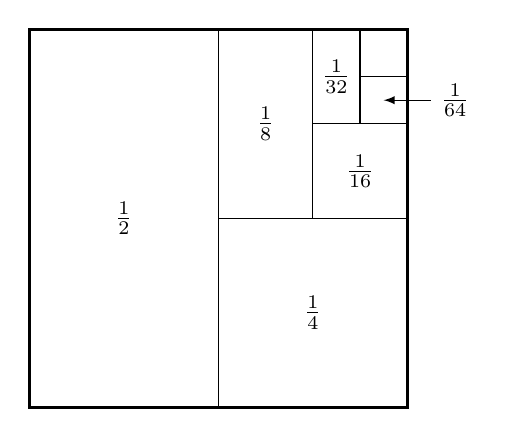
\begin{tikzpicture}[scale=.6,>=latex]
        \draw[very thick] (0,0) rectangle (8,8);
\draw(4,0)--(4,8);  \node at (2,4){$\frac{1}{2}$};
\draw (4,4)--(8,4); \node at (6,2){$\frac{1}{4}$};
\draw (6,4)--(6,8); \node at (5,6){$\frac{1}{8}$};
\draw (6,6)--(8,6); \node at (7,5){$\frac{1}{16}$};
\draw (7,6)--(7,8); \node at (6.5,7){$\frac{1}{32}$};
\draw (7,7)--(8,7); 
\draw[<-] (7.5,6.5)--(8.5,6.5)node[right] {$\frac{1}{64}$};
    \end{tikzpicture}
    \caption{}
\end{figure}

例如:一个单位正方形,每次取它面积的一半,累加起
来,得到无穷级数,(如图7.4)
\[\frac{1}{2}+\frac{1}{4}+\frac{1}{8}+\frac{1}{16}+\frac{1}{32}+\cdots\]
从这个无穷级数里,依次取出前$n$项的部分和$S_n$, 得到数
列$\{s_n\}$:
\[s_1=\frac{1}{2},\quad s_2=\frac{1}{2}+\frac{1}{4}=\frac{3}{4},\quad s_3=\frac{1}{2}+\frac{1}{4}+\frac{1}{8}=\frac{7}{8},\ldots\]
\[s_n=\frac{1}{2}+\frac{1}{4}+\cdots+\frac{1}{2^n}=\frac{\frac{1}{2}\left[1-\left(\frac{1}{2}\right)^n\right]}{1-\frac{1}{2}}=1-\left(\frac{1}{2}\right)^n,\ldots\]

我们看到,这个数列$\{s_n\}$和原正方形的关系是:
\begin{enumerate}
    \item 前$n$项部分和$s_n$小于1;
    \item $s_n$与1的误差$|s_n-1|$, 只要$n$充分大,就可以
小到任意小。
\end{enumerate}
因此,前$n$项部分和$s_n$的极限是1, 即
\[\lim_{n\to\infty} s_n=1 \]

我们可以这样理解无穷级数$\displaystyle\sum_{n=1}^{\infty}\frac{1}{2^n}$的意义,它就是前$n$
项部分和$s_n$的极限值,于是
\[\frac{1}{2}+\frac{1}{4}+\frac{1}{8}+\cdots+\frac{1}{2^n}+\cdots=1 \]
我们说,这个无穷级数收敛到1, 而前$n$项的部分和$s_n$是这
个极限的近似值。

现在,我们可以赋予这一类收敛的无穷级数以和的意义。

\begin{blk}{定义}
    如果无穷级数$u_1+u_2+\cdots+u_n+\cdots$的前$n$项部分
和$s_n$所组成的数列$\{s_n\}$有极限值,即$\Lim_{n\to\infty}s_n=s$, 那么,这个无
穷级数就叫做收敛的,并把这个确定的数$\Lim_{n\to\infty}s_n=s$叫做这个无穷级数的和,即
\[\sum_{n=1}^{\infty}u_n=\Lim_{n\to\infty}s_n=s\]
\end{blk}
 
下面我们用收敛的数列来构造收敛的无穷级数。
假设数列$\{a_n\}$是收敛的,即$\Lim_{n\to\infty}a_n=A$, 令
$b_i=a_i-a_{i-1},\; i=1,2,\ldots$,
即得一个新数列$\{b_n\}$。无穷级数
$b_1+b_2+\cdots+b_n+b_{n+1}+\cdots$是收敛的。

事实上,这个级数的部分和是:
\[\begin{split}
    s_1&=b_1=a_1-a_0\\
    s_2&=b_1+b_2=(a_1-a_0)+(a_2-a_1)=a_2-a_0\\
    s_3&=b_1+b_2+b_3=(a_1-a_0)+(a_2-a_1)+(a_3-a_2)=a_3-a_0\\
    \cdots & \cdots\cdots\cdots\cdots\\
    s_n&=b_1+b_2+\cdots +b_n=(a_1-a_0)+(a_2-a_1)+\cdots +(a_n-a_{n-1})=a_n-a_0\\
    \cdots & \cdots\cdots\cdots\cdots\\
\end{split} \]
因此:
\begin{equation}
    \begin{split}
        \sum^{\infty}_{i=1}b_i&=\lim_{n\to\infty}\sum^n_{i=1}b_i=\lim_{n\to\infty}(a_n-a_0)\\
        &=\lim_{n\to\infty}a_n-a_0
    \end{split}
\end{equation}
因此,无穷级数$\sum^{\infty}_{i=1}b_i$是收敛的。


\begin{example}
令$a_n=1-\frac{1}{n+1}$, $n=0,1,2,\ldots$,显然$\{a_n\}$是收敛的,并且$\Lim_{n\to \infty}a_n=1$。

令\[\begin{split}
    b_i&=a_{i}-a_{i-1}=\left(1-\frac{1}{i+1}\right)-\left(1-\frac{1}{i}\right)\\
    &=\frac{1}{i}-\frac{1}{i+1}=\frac{1}{i(i+1)}
\end{split}\]
于是,      
\[\begin{split}
    \frac{1}{1\cdot 2}+\frac{1}{2\cdot 3}+\frac{1}{3\cdot 4}+\cdots +\frac{1}{n(n+1)}&=\lim_{n\to\infty}a_n-a_0\\
    &=\lim_{n\to\infty}\left(1-\frac{1}{n-1}\right)-0=1
\end{split}\]

上面(7.3)式也表示,要求一个无穷级数的和$\sum^{\infty}_{i=1}b_i$, 常将$b_i$分解,使$b_i=a_i-a_{i-1}$, 于是求无穷级数的和就转化为求
数列$\{a_n\}$的极限。
\end{example}

\begin{example}
    求以下无穷等比级数的和。
    \[a_1+a_q+a_1q^2+\cdots +aq^{n-1}+\cdots \qquad (|q|<1)\]
\end{example}


\begin{solution}
    我们在本章中,已经证明,若$|q|<1$, 则$\Lim_{n\to\infty}q^n=0$。因为:
\[s_n=\frac{a_1(1-q^n)}{1-q}=\frac{a_1}{1-q}-\frac{a_1q^n}{1-q}\]
所以,
\[\Lim_{n\to\infty}s_n=\frac{a_1}{1-q}-\frac{a_1}{1-q}\Lim_{n\to\infty}q^n=\frac{a_1}{1-q}\]
因此:\[a_1+a_q+a_1q^2+\cdots +aq^{n-1}+\cdots=\frac{a_1}{1-q} \quad (|q|<1)\]
\end{solution}

为了讨论循环小数及以后的需要,让我们用下面两个定
理作为本节的总结。

\begin{blk}{定理1}
    无穷等比级数,$\sum^{\infty}_{n=1}a_1q^{n-1}$收敛的充分必要条件是公比$q$的绝对值$|q|<1$, 此时,它的和是$\frac{a_1}{1-q}$, (注意这里$q\ne 1$)。
\end{blk}

\begin{proof}
    上面的例7.17已证明了$|q|<1$是$\sum^{\infty}_{n=1}a_1q^{n-1}=\frac{a_1}{1-q}$
的充分条件。要证必要性,我们只须注意到,如果$|q|\ge 1$, 
那么$a_n=a_1q^{n-1}$是发散的,于是,$\sum^{\infty}_{n=1}a_1q^{n-1}$也是发散的(见下
面的定理2)。
\end{proof}

\begin{blk}{定理2}
无穷级数$\sum^{\infty}_{i=1}a_i$收敛的必要条件是$\Lim_{n\to \infty}a_n=0$.
\end{blk}

\begin{proof}
因为$a_n=(a_1+a_2+\cdots +a_n)-(a_1+a_2+\cdots +a_{n-1})
=s_n-s_{n-1}$

由于$\sum^{\infty}_{i=1}a_i$是收敛的,故有
\[\begin{split}
    \lim_{n\to\infty}s_n&=\lim_{n\to\infty}s_{n-1}=s\\
    \lim_{n\to\infty}a_n&=\lim_{n\to\infty}(s_n-s_{n-1})=\lim_{n\to\infty}s_n-\lim_{n\to\infty}s_{n-1}=s-s=0
\end{split}\]
\end{proof}

下面的例题说明这个条件不是充分的。


\begin{example}
    $\frac{1}{1}+\frac{1}{2}+\frac{1}{3}+\cdots +\frac{1}{n}+\cdots$是发散级数,为什么呢?
\end{example}


\begin{solution}
    我们首先注意到这是正项级数,因此,部分和会越
来越大,而且
\[\begin{split}
    s_1&=1          \\
    s_2&=1+\frac{1}{2}          \\
    s_4&=1+\frac{1}{2}+\frac{1}{3}+\frac{1}{4}>1+\frac{1}{2}+\frac{1}{4}+\frac{1}{4}=1+\frac{1}{2}+\frac{1}{2}          \\
    s_8&=1+\frac{1}{2}+\frac{1}{3}+\frac{1}{4}+\frac{1}{5}+\frac{1}{6}+\frac{1}{7}+\frac{1}{9}          \\
    &>1+\frac{1}{2}+\frac{1}{4}+\frac{1}{4}+\frac{1}{8}+\frac{1}{8}+\frac{1}{8}+\frac{1}{8}=1+\frac{1}{2}+\frac{1}{2}+\frac{1}{2}\\
    \cdots &\cdots \cdots \cdots \cdots 
\end{split}\]

一般地,
\[s_{2^m}=1+\overbrace{\frac{1}{2}+\frac{1}{2}+\cdots +\frac{1}{2}}^{\text{$m$个}}=\frac{m+2}{2}\]    
因为,当$m$无限增大时,$\frac{m+2}{2}$
越来越大毫无止境,故$s_{2^m}$也
发散到无穷大,又总有这样的$n$满足$2^m<n$, 故当$m\to\infty$时,
也使$m\to\infty$, $s_n>s_{2^m}\to \infty$, 即$s_n$也发散到无穷大。

注意到:$a_n\to 0$, 但如果数列$\{s_n\}$中的子数列$\{s_{2^m}\}$是
发散的,那么$\{s_n\}$也是发散的。
\end{solution}

\subsection{无限小数与十分逼近}
在这一节,我们要用无限十进小数来描述实数,要说明
无限小数的意义,证明每一个循环小数都等于一个分数,而
每一个分数都等于一个循环小数。

现在我们借助十分逼近法去规定实数的无限十进小数表
示。考察某实数$x$. 将数轴分为单位线段,各分点均为整数。点
$x$在某一线段内,或者本身就是一个分点。如果$x$是相邻两
个单位线段的分点,约定$x$属于线段的左端点。于是,存在
一个整数$\alpha_0$,使得
\[\alpha_0\le x<\alpha_0+1,\quad \text{即}\; x\in \overline{A_0B_0}=(\alpha_0,\alpha_0+1)\]

$\alpha_0+\frac{1}{10},\; \alpha_0+\frac{2}{10},\; \alpha_0+\frac{3}{10},\;\ldots,\; \alpha_0+\frac{9}{10}$
这些点将
$\overline{A_0B_0}=(\alpha_0,\alpha_0+1)$分为十等份,点$x$必在某一个分段内,或
者$x$本身是一个分点,如果是分点,约定$x$属于分段的左端
点,在这两种情况下,存在一个整数$\alpha_1,\; (0\le \alpha_1\le 9)$, 使得
\[\alpha_0+\frac{\alpha_1}{10}\le x<\alpha_0+\frac{\alpha_1+1}{10}\]
即:$x\in\overline{A_1B_1}=\left[\alpha_0+\frac{\alpha_1}{10}, \alpha_0+\frac{\alpha_1+1}{10}\right)$。

再将线段$\overline{A_1B_1}$十等分,我们可以找到一个整数$\alpha_2$($0\le \alpha_2\le 9$),使得
\[\alpha_0+\frac{\alpha_1}{10}+\frac{\alpha_2}{10^2}\le x<\alpha_0+\frac{\alpha_1+1}{10}+\frac{\alpha_2+1}{10^2}\]
即:$x\in\overline{A_2B_2}=\left[\alpha_0+\frac{\alpha_1}{10}+\frac{\alpha_2}{10^2}, \alpha_0+\frac{\alpha_1+1}{10}+\frac{\alpha_2+1}{10^2}\right)$。

经过$n$步以后,$x$必在线段$\overline{A_nB_n}$之中,即
\[\alpha_0+\frac{\alpha_1}{10}+\frac{\alpha_2}{10^2}+\cdots+\frac{\alpha_n}{10^n}\le x<\alpha_0+\frac{\alpha_1}{10}+\frac{\alpha_2}{10^2}+\cdots+\frac{\alpha_n+1}{10^n}\]
这里$\alpha_1,\alpha_2,\ldots,\alpha_n$都是0到9之间的整数,线段$\overline{A_nB_n}$之
长度等于$\frac{1}{10^n}$
,而有限十进小数$\alpha_0.\alpha_1\alpha_2\cdots\alpha_n$和$\alpha_0,\alpha_1\alpha_2\cdots(\alpha_n+1)$分别是$x$的准确到
$\frac{1}{10^n}$
的不足近似值和过剩近似值。

让这个十分逼近过程无限地进行下去,那么实数$x$就完
全可以由无限小数$\alpha_0.\alpha_1\alpha_2\cdots\alpha_n\cdots$来表示,同时由于$x$与有限
小数近似值的误差
\[|\alpha_0.\alpha_1\alpha_2\cdots\alpha_n-x|<\frac{1}{10^n},\qquad  |\alpha_0.\alpha_1\alpha_2\cdots(\alpha_n+1)-x|<\frac{1}{10^n}\]
当$n$充分大时,可以小到任意小,所以无
限小数$x=\alpha_0.\alpha_1\alpha_2\cdots\alpha_n\cdots$是由有限十进小数组成的两个数列:
\[\alpha_0,\; \alpha_0.\alpha_1,\;\alpha_0.\alpha_1\alpha_2,\;\ldots,\;  \alpha_0.\alpha_1\alpha_2\cdots\alpha_n,\;\ldots\]
与
\[(\alpha_0+1),\; \alpha_0.(\alpha_1+1),\;\alpha_0.\alpha_1(\alpha_2+1),\;\ldots, \alpha_0.\alpha_1\alpha_2\cdots(\alpha_n+1),\;\ldots\]
的共同的极限值。

\textbf{无限小数的定义}是这样的,我们取实数的小数点以下第
$n$位为止的有限小数$\alpha_0.\alpha_1\alpha_2\cdots\alpha_n$,记作$x_n$, 即$x_n=\alpha_0.\alpha_1\alpha_2\cdots\alpha_n$,那么数列$\{x_n\}$的极限值是这个无限小数,用式子表示
就是
\[\lim_{n\to\infty}x_n=x=\alpha_0.\alpha_1\alpha_2\cdots\alpha_n\cdots\]


\begin{example}
$\frac{2}{3}=0.\dot{6}$表示数列$\{x_n\}$的极限:
\[x_1=0.6,\; x_2=0.66,\; x_3=0.666,\ldots,\; x_n=0.\underbrace{66\cdots 66}_{\text{$n$位小数}},\; \ldots\]
\end{example}

\begin{example}
    无限小数$\pi=3.1415926\cdots$
    的意思是,令
   \[ x_1=3.1,\; x_2=3.14,\; x_3=3.141,\; \ldots\]
    那么$x_n\to \pi$。
\end{example}

    注意,在上面我们用十分逼近得到实数$x$的无限十进小
    数表示时,在$x$是十等分的一个分点的情形,如果不限定$x$
    属于两相邻线段的左端点,那么对于同一个整数或有限小
    数,可能有两类不同的无限十进小数表示法。例如
\[1=1.0000\cdots=0.999\cdots,\quad 2.35=2.35000\cdots=2.34999\cdots\]

    为排除这种不确定性,按照我们的约定,就可以去掉那
    些从某一位以后有数字都是9的十进小数表达式。

把实数写成小数形式,便于比较它们的大小。在比较
时,遇到以9为循环节结尾的无限小数都用以0为循环节结
尾的无限小数代替。

今有两个实数
$x=\alpha_0.\alpha_1\alpha_2\cdots\alpha_n\cdots$ 和$y=\beta_0.\beta_1\beta_2\cdots\beta_n\cdots$,
比较这两个实数$x$和$y$的大小,只须比较两个数的各数位上
的数字,并且注意在哪一个数位上的数字不同,从而告诉我
们哪个实数大。


例如:$\frac{17}{20}=0.850000\cdots$, $\frac{45}{53}=0.84905000\cdots$,
看一眼就能发觉,它们有相同的第一位小数,
$\frac{17}{20}$的 第二位小数大
于$\frac{45}{53}$的第二位小数,因此,
$\frac{17}{20}>\frac{45}{53}$。

一般地,我们说$x>y$, 如果下面的条件中有一个成立
\begin{enumerate}
    \item $\alpha>\beta$
    \item $\alpha=\beta$,而$\alpha_1>\beta_1$
    \item $\alpha=\beta, \alpha_1 =\beta_1,\ldots,\alpha_{\ell}=\beta_{\ell}$,而$\alpha_{\ell+1}>\beta_{\ell+1}$
\end{enumerate}

根据前面的讨论,我们知道任何一个实数都是两个有限
十进小数的夹逼数列的极限。

设$\lim x_n=x=\lim x'_n,\quad \lim y_n=y=\lim y'_n$,
或者
\[x_n\to x\leftarrow x'_n,\qquad y_n\to y\leftarrow y'_n\]
\[x'_n-x_n\to 0,\qquad y'_n-y_n\to 0\]
则对应数列的相加,我们有实数的相加,对应于数列相乘,
我们有实数的相乘,也就是说:
\[\begin{split}
    \lim(x_n+y_n)&=x+y=\lim(x'_n+y'_n)\\
    \lim(x_n\cdot y_n)&=x\cdot y=\lim(x'_n\cdot y'_n)
\end{split}
\]

例如$\sqrt{2}=1.4142135\cdots,\quad \sqrt{3}=1.7320508\cdots$,
\[\begin{cases}
    x_n+y_n\\  x'_n+y'_n
\end{cases}\qquad \begin{cases}
    1.4+1.7=3.1 \\ 1.5+1.8=3.3
\end{cases}\]
\[\begin{cases}
    1.41+1.73=3.14\\1.42+1.74=3.16
\end{cases}\qquad \begin{cases}
    1.414+1.732=3.146\\1.415+1.733=3.148
\end{cases}\]
\[\begin{cases}
    1.4142+1.7320=3.1462\\
1.4143+1.7321=3.1464
\end{cases}\qquad \begin{cases}
    1.41421+1.73205=3.14626\\
1.41422+1.73206=3.14628
\end{cases}\cdots\]
即:
$3.1 <3.14<3.146<3.1462<3.14626<\cdots <\sqrt{2}+\sqrt{3}<\cdots <3.14628<3.1464<3.148<3.16<3.3$

$\therefore\quad \sqrt{2}+\sqrt{3}=3.1462\cdots$。只要把$\sqrt{2}$, $\sqrt{3}$的夹逼小数求到足够多的数位,我们用上
面的方法就可以把$\sqrt{2}+\sqrt{3}$的小数表示求到任意的数
位上。

同样地得到
\[\begin{cases}
    x_n\cdot y_n\\  x'_n\cdot y'_n
\end{cases}\qquad \begin{cases}
    1.4\x 1.7=2.38 \\ 1.5\x 1.8=2.70
\end{cases}\qquad \begin{cases}
    1.41\x 1.73=2.4393\\1.42\x 1.74=2.4708
\end{cases}\]
\[\begin{cases}
    1.414\x 1.732=2.449048\\1.415\x 1.733=2.452195
\end{cases}\qquad \begin{cases}
    1.4142\x 1.7320=2.4493944\\
1.4143\x 1.7321=2.449709
\end{cases}\cdots\]

$\therefore\quad \sqrt{6}=2.449\cdots$。

在无限小数中,除了有一类\textbf{无限循环小数},还有一类\textbf{无
限不循环小数},譬如,$0.1001000100001\cdots$,
就是一个无限不循环小数。

现在我们要来证明每一个循环小数都等于一个分数,而
每一个分数都等于一个循环小数。先举几个将无限循环小数
化为分数的例子,再给出一般的证明。


\begin{example}
    怎样将循环小数$0.\overline{621}$化成分数?
\end{example}

\begin{solution}
    我们可以将无限小数$0.\overline{621}$表示成一个无穷级数
\[\begin{split}
0.\overline{621}&=0.621+0.000621+0.000000621+\cdots\\
&=\frac{621}{10^3}+\frac{621}{10^6}+\frac{621}{10^9}+\cdots
\end{split}\]
显然,这个无穷级数是无穷等比级数,它的首项$a_1=\frac{621}{10^3}$, 公比$q=\frac{1}{10^3}$
根据4.1中的定理,这个无穷等比级数的和是$\frac{a_1}{1-q}$,因此:
\[\begin{split}
    0.\overline{621}&=\frac{621}{10^3}+\frac{621}{10^6}+\frac{621}{10^9}+\cdots\\
    &=\frac{621}{10^3}\cdot \frac{1}{1-\frac{1}{10^3}}=\frac{621}{10^3}\cdot \frac{10^3}{10^3-1}\\
    &=\frac{621}{999}=\frac{23}{37}
\end{split}\]
\end{solution}

\begin{example}
试将$0.3\overline{12}$化成分数。
\end{example}

\begin{solution}
\[\begin{split}
    0.3\overline{12}&= 0.3+0.0\overline{12}=0.3+(0.012+0.00012+\cdots)\\
    &=\frac{3}{10}+\left(\frac{12}{10^3}+\frac{12}{10^5}+\cdots\right)\\
    &=\frac{3}{10}+\frac{12}{10^3}\cdot \frac{1}{1-\frac{1}{10^2}}\\
    &=\frac{3}{10}+\frac{12}{10^3}\cdot \frac{10^2}{10^2-1}\\
    &=\frac{3}{10}+\frac{12}{10}\cdot \frac{1}{99}=\frac{309}{990}=\frac{103}{330}
\end{split}\]
\end{solution}

下面,我们来证明任何一个循环小数一定是一个
分数。

如果$a$是个循环小数,它的循环节是由第$k+1$位开始到
$k+\ell$位,平常我们写作
\[a=a_0.c_1c_2\cdots c_k\overline{c_{k+1}c_{k+2}\cdots c_{k+\ell}}\]
它的意思是
\[\begin{split}
    a&=a_0+\frac{c_1}{10}+\frac{c_2}{10^2}+\cdots +\frac{c_k}{10^k}+\frac{c_{k+1}}{10^{k+1}}+\cdots+\frac{c_{k+\ell}}{10^{k+\ell}}\\
&\qquad +\frac{c_{k+1}}{10^{k+\ell+1}}+\cdots+\frac{c_{k+\ell}}{10^{k+2\ell}}+\frac{c_{k+1}}{10^{k+2\ell+1}}+\cdots+\frac{c_{k+\ell}}{10^{k+3\ell}}+\cdots
\end{split}\]

虽然,这不是无穷等比级数,现在用结合律来构造这个无穷级数的部分和的子数列:

设$S_1=a_0+\frac{c_1}{10},\quad S_2=a_0+\frac{c_1}{10}+\frac{c_2}{10^2},\ldots$ 于是第$k$个部
分和是
\[S_k=a_0+\frac{c_1}{10}+\frac{c_2}{10^2}+\cdots+\frac{c_k}{10^k}\]
再令
\[d=\frac{c_{k+1}}{10^{k+1}}+\frac{c_{k+2}}{10^{k+2}}+\cdots +\frac{c_{k+\ell}}{10^{k+\ell}}\]
所以,$d$是分数,而且$0\le d<1$

那么,第$k+m\ell$个部分和是
\[\begin{split}
    S_{k+m\ell}&=S_k+d+\frac{d}{10^{\ell}}+\frac{d}{10^{2\ell}}+\cdots \frac{d}{10^{(m-1)\ell}}\\
    &=S_k+d\left(1+\frac{1}{10^{\ell}}+\frac{1}{10^{2\ell}}+\cdots +\frac{1}{10^{(m-1)\ell}}\right)\\
    &=S_k+\frac{d\left(1-\frac{1}{10^{m\ell}}\right)}{1-\frac{1}{10^{\ell}}}
\end{split}\]
当$m=1,2,3,\ldots$时,部分和$S_{k+m\ell}$就构成无穷级数的部分
和数列$\{S_n\}$的子数列$\{S_{k+m\ell}\}$, 并且
\[\begin{split}
    \lim_{m\to\infty}S_{k+m\ell}&= \lim_{m\to\infty}\left\{S_k+\frac{d\left(1-\frac{1}{10^{m\ell}}\right)}{1-\frac{1}{10^{\ell}}}\right\}\\
    &=S_k+\frac{d}{1-\frac{1}{10^{\ell}}}=S_k+\frac{10^{\ell}\cdot d}{10^{\ell}-1}=a'
\end{split}\]
这里$a'$表示分数。
我们只证明了部分和数列的子数列$\{S_{k+m\ell}\}$收敛到分数
$a'$, 还需要证明部分和数列$\{S_n\}$也收敛到$a'$.

我们只须注意到原来的循环小数所代表的无穷级数也都
是正项的,这就是说,部分和数列$\{S_n\}$是递增数列,特别
地,如果$k+m\ell\le n<k+(m+1)\ell$,
那么$S_{k+m\ell}\le S_n\le S_{k+(m+1)\ell}$,因此,如果“子数列”$\{S_{k+m\ell},\; m=1,2,3,\ldots\}$
收敛到$a'$, 原数列$\{S_n\}$也收敛到$a'$.

我们已证明了,每个循环小数都可以化为分数,现在证明分
数可以化为循环小数。

设$\frac{a}{b}$为一任意给定的不可约真分数(亦即$a,b$互质且
$a<b$)。
\begin{enumerate}
    \item $b$只含有2或5的质因子,则容易看出
可以化$\frac{a}{b}$
成有限位小数。

事实上,设$b=2^{\alpha}5^{\beta}$, $d=5^{\alpha-\beta}a$, 若$\alpha\ge \beta$,则
$$\frac{a}{b}=\frac{a}{2^{\alpha}5^{\beta}}=\frac{5^{\alpha-\beta}a}{10^{\alpha}}=\frac{d}{10^{\alpha}}$$
为$\alpha$位小数。我们可以把有限位小数看成循环
小数的特例。如:
\[\frac{1237}{2\x 5^3}=\frac{1237\x 2^2}{10^3}=4.948=4.948\overline{0}\]

\item 设$b$与10互质,即:$(b,10)=1$, 根据整数分解的唯一性而知
$\frac{a}{b}$不可能写成$\frac{m}{10^k}$
的形式,这里$m$为正整数,故$\frac{a}{b}$
不可能化为有限小数。做除法,我们得到
\[10a=bq_1+r_1,\qquad 0<r_1<b\]
两边再除以$b$, 得
\[\frac{10a}{b}=q_1+\frac{r_1}{b},\qquad 0<\frac{r_1}{b}<1\]

这里$q$是$0,1,2,\ldots,9$这十个整数中的某个。用
和上面同样的方法,逐步得到
\[\begin{split}
    \frac{10r_1}{b}&=q_2+\frac{r_2}{b},\qquad 0<\frac{r_2}{b}<1,\\
    \frac{10r_2}{b}&=q_3+\frac{r_3}{b},\qquad 0<\frac{r_3}{b}<1,\\
\cdots &\cdots \cdots \cdots \cdots \\
    \frac{10r_{n-1}}{b}&=q_n+\frac{r_n}{b},\qquad 0<\frac{r_n}{b}<1\\
\end{split}\]
这里每个$q_n$是$0,1,2,\ldots,9$这十个整数中的某个,
于是
\[\begin{split}
    \frac{a}{b}&=\frac{q_1}{10}+\frac{r_1}{10b}\\
    &=\frac{q_1}{10}+\frac{q_2}{10^2}+\frac{r_2}{10^2b}\\
    &=\frac{q_1}{10}+\frac{q_2}{10^2}+\frac{q_3}{10^3}+\frac{r_3}{10^3b}\\
    \cdots &\cdots \cdots \cdots \cdots \\
    &=\frac{q_1}{10}+\frac{q_2}{10^2}+\cdots+\frac{q_n}{10^n}+\frac{r_n}{10^n b}\\
\end{split}\]

再设
\[\begin{split}
    x_n&=\frac{q_1}{10}+\frac{q_2}{10^2}+\cdots+\frac{q_n}{10^n}\\
    y_n&=\frac{q_1}{10}+\frac{q_2}{10^2}+\cdots+\frac{q_n+1}{10^n}\\
    d_n&=\frac{r_n}{10^n b}<\frac{1}{10^n}
\end{split}\]
则:
\[\frac{a}{b}=x_n+d_n,\qquad 0<d_n<\frac{1}{10^n}\]

再有$x_1<x_2<\cdots<x_{n-1}<x_n<\cdots<y_n<y_{n-1}<\cdots<y_2<y_1$,且$y_n-x_n\to 0$。

当$n$无限增大时,根据实数完备性,无限小数
\[\sum_{n=1}^{\infty}\frac{q_n}{10^n}=0.q_1q_2\cdots q_n\cdots\]
表示一实数,又因为,$d_n\to 0$, 故我们确定了一
个其值为$\frac{a}{b}$
的无限小数$0.q_1q_2\cdots q_n\cdots$。

再说明这个无限小数一定是纯循环小数,设$a=r_0$, 因为
$r_0,r_1,r_2,\ldots,r_n,\ldots$是一串大于0而小于$b$的正整数,这种正
整数只有$b-1$个不同的,所以,这一串数$r_0=a,r_1,r_2,\ldots r_n,\ldots$必然有二者会相同,就假定$r_k$为首先出现的重见余
数,假定这两个相同的余数是$r_k$和$r_i$, 即有$r_k=r_i$. 现在我
们要证明$r_i$只能是$a=r_0$, 用反证法,若$i>0$则由等式
$\frac{10r_{k-1}}{b}=q_k+r_k$和$\frac{10r_{i-1}}{b}=q_i+r_i$ 两边作减法,得到
\[\frac{10(r_{k-1}-r_{i-1})}{b}=q_k-q_i\]
因为$q_k-q_i$是整数,所以$b$能整除$10(r_{k-1}-r_{i-1})$, 由于$b$与10
互质,故$b$能整除$r_{k-1}-r_{i-1}$,但是$r_{k-1}-r_{i-1}<b$, 所以$r_{k-1}-r_{i-1}=0$, 即$r_{k-1}=r_{i-1}$重见更早,与原设$r_k$为首先出现的重
见余数不合,故$i=0$。

$\therefore\quad r_k=r_0=a$, 这样
\[\frac{a}{b}=0.\overline{q_1q_2\cdots q_{k-1}q_k}\]

\item 设$b=2^{\alpha}5^{\beta}b_1$, 而$b_1>1$且与10互质,又$\alpha$与$\beta$均不
为0, 若$\alpha\ge \beta$,
\[\frac{a}{b}=\frac{a}{2^{\alpha}5^{\beta}b_1}=\frac{5^{\alpha-\beta}a}{10^{\alpha}b_1}\]
做$5^{\alpha-\beta}a$除以$b_1$, 得
\[5^{\alpha-\beta}a=M{b_1}+{r},\quad 0<r<b\]
$M$是一个正整数,两边再除
以$b_1$, 得
\[5^{\alpha-\beta}\frac{a}{b_1}=M+\frac{r}{b_1},\qquad 0<\frac{r}{b_1}<1\]
由前段证明2的结果
\[\frac{r}{b_1}=0.\overline{c_1c_2\cdots c_{s}}\]
故,
\[\begin{split}
    \frac{a}{b}&=\frac{5^{\alpha-\beta}a}{10^{\alpha}b_1}=\frac{1}{10^{\alpha}}\left(M+0.\overline{c_1c_2\cdots c_{s}}\right)\\
    &=\frac{1}{10^{\alpha}}\left(M.\overline{c_1c_2\cdots c_{s}}\right)
\end{split}\]

当以$10^{\alpha}$除以$M.\overline{c_1c_2\cdots c_{s}}$时,也就是将小数点左移$\alpha$位,我们得到
\[\frac{a}{b}=0.m_1m_2\cdots m_{\alpha}\overline{c_1c_2\cdots c_{s}}\]
为混循环小数。
\end{enumerate}

若$\alpha\le \beta$, 可以用同样的方法说明$\frac{a}{b}$
为一混循环小数,因
此有
\begin{blk}{定理}
    任何一个分数都等于某一个循环小数,任何一个
循环小数必然是个分数。
\end{blk}

如果采用无限十进小数来描述实数,我们按照下表来对
实数分类:
\[\text{实数——无限十进小数}\begin{cases}
    \text{有理数—无限十进循环小数}\\
    \text{无理数—无限十进不循环小数}
\end{cases}\]

\section*{习题7.4}
\addcontentsline{toc}{subsection}{习题7.4}
\begin{enumerate}
    \item 求下列无穷等比数列的和:
    \begin{multicols}{2}
\begin{enumerate}
    \item $\frac{1}{2}+\frac{1}{3}+\frac{2}{9}+\cdots$
    \item $1-\frac{2}{5}+\frac{4}{25}-\cdots$
    \item $\sqrt{\frac{3}{2}}+\sqrt{\frac{2}{3}}+\frac{2}{3}\sqrt{\frac{2}{3}}+\cdots$
    \item $\frac{\sqrt{3}+1}{\sqrt{3}-1}+1+\frac{\sqrt{3}-1}{\sqrt{3}+1}+\cdots$
\end{enumerate}        
    \end{multicols}


\item 若$a,b$是实数且$\left|\frac{a+2b+3}{b+3}\right|+3(a+3b)^2=0$, 求等比级数$ab+b+\frac{b}{a}+\cdots$的和。
\item 已知$\sqrt{3}\sin\alpha-\cos\alpha=0$, $\alpha$为锐角,
求$\sum^{\infty}_{n=0}(-\sin\alpha)^n$

\item 求下列无穷级数的和:
\begin{enumerate}
\item $\frac{1}{1 \times 4}+\frac{1}{2 \times 5}+\frac{1}{3 \times 6}+\frac{1}{4 \times 7}+\cdots$
\item $\frac{6}{2 \times 7}+\frac{6}{7 \times 12}+\frac{6}{12 \times 17}+\frac{6}{17 \times 22}+\cdots$
\item $\frac{1}{1 \times 2 \times 3}+\frac{1}{2 \times 3 \times 4}+\frac{1}{3 \times 4 \times 5}+\frac{1}{4 \times 5 \times 6}+\cdots$
\item $\frac{1}{1 \times 2 \times 3 \times 4}+\frac{1}{2 \times 3 \times 4 \times 5}+\frac{1}{3 \times 4 \times 5 \times 6}+\frac{1}{4 \times 5 \times 6 \times 7}+\cdots$
\item $\frac{1}{7}+\frac{2}{7^{2}}+\frac{3}{7^{3}}+\frac{1}{7^{4}}+\frac{2}{7^{6}}+\frac{3}{7^{6}}+\frac{1}{7^{7}}+\frac{2}{7^{8}}+\frac{3}{7^{9}}+\cdots$
\end{enumerate}


\item 求下列各式的极限值:
\begin{enumerate}
    \item  $\Lim _{n\to  \infty} \frac{1+a+a^{2}+\cdots+a^{n}}{1+b+b^{2}+\cdots+b^{n}} \qquad(|a|<1,\;|b|<1)$
    \item  $\Lim _{n\to  \infty}\left(\frac{1}{n}-\frac{2}{n}+\frac{3}{n}-\cdots+\frac{(-1)^{n-1} n}{n}\right)$
    \item $\Lim _{n\to  \infty}\left(\frac{1^{2}}{n^{3}}+\frac{2^{2}}{n^{3}}+\cdots+\frac{(n-1)^{2}}{n^{3}}\right)$
    \item $\Lim _{n\to  \infty}\left(\frac{1}{2}+\frac{3}{{2^2}}+\frac{5}{2^3}+\cdots+\frac{2n-1}{2^{n}}\right)$
\end{enumerate}

\item $\Lim _{n\to  \infty}\left(1-\frac{1}{2^2}\right)\left(1-\frac{1}{3^2}\right)\left(1-\frac{1}{4^2}\right)\cdots\left(1-\frac{1}{n^2}\right)$

\item 数列$x_n\; (n=1,2,3,\ldots)$是由下列各式所确定:
\[x_0=a,\; x_1=b,\; x_n=\frac{x_{n-2}+x_{n-1}}{2}\quad (n\ge 2)\]
求$\Lim_{n\to\infty}x_n$.

\item 将下列循环小数化为分数:
\[0.\overline{47},\qquad 2.\overline{234},\qquad 0.4\overline{7},\qquad 3.2\overline{31},\qquad 0.\overline{1108},\qquad 5.38\overline{90}\]
\item 求出下列各式的值:
\begin{enumerate}
    \item $0.\overline{48}\x0.\overline{48}$
    \item $0.\overline{12}+0.\overline{83}+0.\overline{34}+\cdots+0.\overline{89}$
    \item $0.\overline{15}+0.0\overline{15}+0.00\overline{15}+\cdots$
\end{enumerate}
\end{enumerate}

\section{数列极限在几何上的应用}
在平面几何中,我们知道了什么是相似形,而且知道研
究相似形的基本定理是“设$\triangle ABC$和$\triangle A'B'C'$的三个内角对
应相等,则其对应边长成比例”。在初中时,我们证明了当比值
是有理数时,定理是对的,现在要补充推证,在比值是无理
数时,定理也是对的,这样这个定理的证明才是完整的。

\begin{proof}
设$AB=kA'B'$, 这里$k$是无理数,我们要证明
\[\frac{AC}{A'C'}=\frac{BC}{B'C'}=k\]
我们知道任何一个无理数可以用有理数
来逼近,于是可以找到两串有理数$k'_n,k''_n$从左、右夹逼无理
数$k$使得
\[k'_n\to k\leftarrow k''_n,\quad \text{或者}\quad \lim_{n\to\infty}k'_n=\lim_{n\to\infty}k''_n=k\]
比如,$k$是特殊的情形,$k=\sqrt{2}$,则可取
\[\begin{split}
    k'_1&=1,\quad     k'_2=1.4,\quad    k'_3=1.41,\;\ldots\\ 
    k''_1&=1,\quad     k''_2=1.5,\quad    k''_3=1.42,\;\ldots\\
\end{split}\]

\begin{figure}[htp]
    \centering
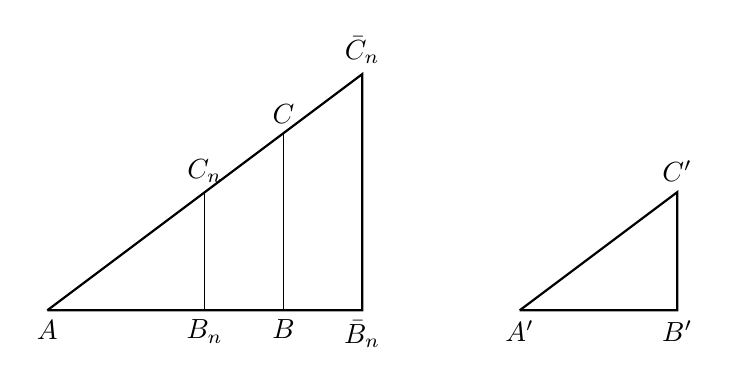
\begin{tikzpicture}
\begin{scope}
    \draw[thick] (0,0)node[below]{$A$}--(4,0)node[below]{$\bar{B}_n$}--(4,3)node[above]{$\bar{C}_n$}--(0,0);
    \draw(3,0)node[below]{${B}$}--(3,2.25)node[above]{$C$};
    \draw(2,0)node[below]{${B}_n$}--(2,1.5)node[above]{${C}_n$};
\end{scope}
\begin{scope}[xshift=6cm]
\draw[thick] (0,0)node[below]{$A'$}--(2,0)node[below]{$B'$}--(2,1.5)node[above]{$C'$}--(0,0);
\end{scope}
\end{tikzpicture}
    \caption{}
\end{figure}

如图7.5,在直线$AB$上取点列$\{B_n\}$和$\{\bar{B}_n\}$使得
\[AB_n=k'_nA'B',\qquad A\bar{B}_n=k''_n A'B'\]
再由$B_n$, $\bar{B}_n$点分别作$BC$边平行线交$AC$线于$C_n$, $\bar{C}_n$点,则因
为相似三角形定理对有理数比值是对的,所以
\[\triangle AB_nC_n\backsim \triangle A\bar{B}_n\bar{C}_n\backsim \triangle A'B'C'\]
\[\begin{split}
    \frac{AB_n}{A'B'}&=\frac{AC_n}{A'C'}=\frac{B_nC_n}{B'C'}=k'_n\\
    \frac{A\bar{B}_n}{A'B'}&=\frac{A\bar{C}_n}{A'C'}=\frac{\bar{B}_n\bar{C}_n}{B'C'}=k''_n\\
\end{split}\]
由作图知
\[k'_nA'B'=AB_n<AB<A\bar{B}_n=k''_nA'B'\]
并可得
\[\begin{split}
     k'_nA'C'&=AC_n<AC<A\bar{C}_n=k''_nA'C'\\
k'_nB'C'&=B_nC_n<BC<\bar{B}_n\bar{C}_n=k''_nB'C'
\end{split}\]
对上面不等式各端取极限,得到
\[\lim_{n\to\infty} k'_n A'C'  =  \lim_{n\to\infty}k''_n A'C'   =kA'C'\]
另一方面又可得到
\[\lim_{n\to\infty} k'_n A'C' = \lim_{n\to\infty}k''_n A'C'  =AC\]
根据数列的极限值是唯一的,因此$AC=kA'C'$, 同理可得
$BC=kB'C'$。
\end{proof}

总结上面的证明可以归纳成下面两点:
\begin{enumerate}
    \item 先有一个数$k$, 因为它是无理数,比较复杂,往
往我们要用简单的有理数逐步逼近它;
\item 在求极限过程中,要点是要用极限值的唯一性保
证所要的结论。
\end{enumerate}

在几何上,$\pi$表示单位圆的面积,这个面积 显然能用一
个有理数或无理数来表示,可是,如果我们想要以任何精确
度计算出数元,这个定义对于我们来说并没有什么帮助。这
时,我们必须借助于求极限的过程,把数$\pi$表示为已知并且
不难算出的数列的极限,除此外别无它法。

假如我们把单位圆等分成$2n$个小扇形,然后一上一下间
插排列起来,如图7.6.
\begin{figure}[htp]
    \centering
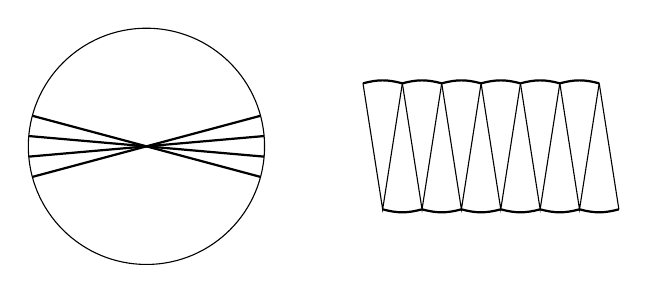
\begin{tikzpicture}
\begin{scope}
    \draw (0,0) circle (1.5);
    \foreach \x in {15,-5,5,-15}
    {
        \draw[thick] (\x:1.5)--(\x+180:1.5);
    }
    
\end{scope}

\begin{scope}[xshift=3cm]
    \foreach \x in {0,.5,1,...,2.5}
    {
        \draw[thick] (\x,-.8) to[bend right=15] (\x+.5,-.8);
        \draw[thick] (\x-.25,.8) to[bend right=-15] (\x+.25,.8);
        \draw[smooth] (\x+.25,.8)--(\x,-.8)--(\x-.25,.8) ;
    }
    \draw[smooth] (3,-.8)--(3-.25,.8) ;
\end{scope}
\end{tikzpicture}
    \caption{}
\end{figure}

当$n$愈大时,上图就愈接近一个高为1, 面积为$\pi$的矩形。
这也就说明了单位圆的圆周长等于$2\pi$。

早在三国时代,我国古代数学家刘徽于公元263年在《九
章算术》中,对古率$\pi=3$极为不满,就提出了用折线逐步地来
逼近曲线,用正多边形的面积来逐步地逼近圆的面积的思
想,他说如果圆内接正六边形,正十二边形,二十四边形……
依次递求它的面积,边数愈增多则其面积与圆面积 愈加接
近,如果边数增加到无限则多边形面积的极限就与圆面积
相等。

设$\pi$为单位圆面积,$S_n$为单位圆的内接正$n$边形的面
积,$S$为单位圆的外切正$n$边形的面积,如图7.7, 对于每一
个$n$, 从几何直观上作如下估计
\begin{figure}[htp]
    \centering
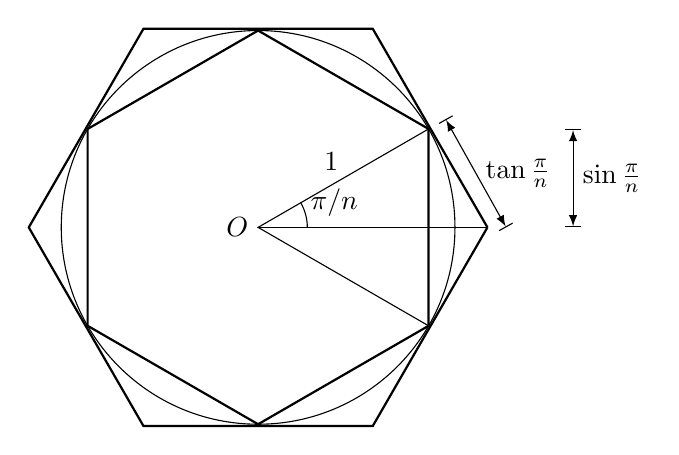
\begin{tikzpicture}[>=latex, scale=2.5]
\draw (0,0) circle (1);
\draw[thick] (30:1)--(90:1)--(150:1)--(210:1)--(270:1)--(330:1)--(30:1);
\draw [thick](0:1.165)--(60:1.165)--(120:1.165)--(180:1.165)--(240:1.165)--(300:1.165)--(0:1.165);
\draw (0,0)node[left]{$O$}--(0:1.165);
\draw  (-30:1)--(0,0)-- (30:1);

\draw[|<->|] (1.6,0) --node[right]{$\sin\frac{\pi}{n}$}(1.6,.5);
\draw (.25,0) arc (0:30:.25)node[right]{$\pi/n$}; 
\draw[|<->|] (1.26,0) --node[right]{$\tan\frac{\pi}{n}$}(30:1.1);
\node at (42:.5){1};
\end{tikzpicture}   
    \caption{}
\end{figure}

$S_n<S_{2n}<\pi<S'_{2n}<S'_n$, 
刘徽的计算理论基础是,
$|S_n-\pi|<S'_n-S_n$, 在$n$无限增大时,$(S'_n-S_n)\to 0$. 从
图7.7看出:
\[\begin{split}
    S'_n&=2n\text{直角三角形的面积}=2n\cdot \frac{1}{2}\tan\frac{\pi}{n}=n\tan\frac{\pi}{n}   \\
    S_n&=2n\text{直角三角形的面积}=2n\cdot \frac{1}{2}\cos\frac{\pi}{n}\cdot \sin \frac{\pi}{n}=n\sin\frac{\pi}{n}\cdot \cos\frac{\pi}{n}
\end{split}\]

\[\begin{split}
    S'_n-S_n &= n\left(\tan\frac{\pi}{n}-\sin\frac{\pi}{n}\cdot \cos\frac{\pi}{n}\right)\\
    &=n \sin\frac{\pi}{n}\left(\frac{1}{\cos\frac{\pi}{n}}-\cos\frac{\pi}{n}\right)\\
    &=\frac{1}{2}(\text{圆内接$n$边形周长})\left(\frac{1}{\cos\frac{\pi}{n}}-\cos\frac{\pi}{n}\right)\\
    &<\frac{1}{2}(\text{圆外切六边形周长})\left(\frac{1}{\cos\frac{\pi}{n}}-\cos\frac{\pi}{n}\right)\to 0\\
\end{split} \]

这就说明了由圆内接正多边形的面积所组成的数列
$\{S_{6\cdot 2^{n-1}}\}$的极限是$\pi$. 

让我们计算这个数列中的前面几个面积。面积的通项是
\[S_{6\cdot 2^{n-1}}=6\cdot 2^{n-1}\left(\frac{1}{2}\sin\frac{\pi}{3\cdot 2^{n-1}}\right)=3\cdot 2^{n-1}\sin\frac{\pi}{3\cdot 2^{n-1}}\quad (n=1,2,3,\ldots)\]

为由$\sin\frac{\pi}{n}$求出$\sin\frac{\pi}{2n}$, 我们需要导出它们之间的递推关系:
\[\begin{split}
    \sin\frac{\pi}{2n}&=\sqrt{\frac{1-\cos\frac{\pi}{n}}{2}}\\
    &=\frac{1}{2}\sqrt{2-2\cos\frac{\pi}{n}}\\
    &=\frac{1}{2}\sqrt{2-2\sqrt{1-\sin^2\frac{\pi}{n}}}
\end{split}\]
于是:
\begin{itemize}
    \item 当$n=1$, $S_6=3\cdot \sin \frac{\pi}{3}=2.5980762$, 
    \item 当$n=2$, $S_{12}=6\cdot \sin \frac{\pi}{6}=3$,
    \item 当$n=3$, 
    \[\begin{split}
        S_{24}&=12\cdot \sin \frac{\pi}{12}=12\left(\frac{1}{2}\sqrt{2-2\sqrt{1-\left(\frac{1}{2}\right)^2}}\right)\\
        &=12\cdot \left(\frac{1}{2}\sqrt{2-\sqrt{3}}\right)=12\x 0.258819=3.1058285
    \end{split}\]
    \item 当$n=4$, 
    \[\begin{split}
        S_{48}&=24\cdot \sin \frac{\pi}{24}=24\left(\frac{1}{2}\sqrt{2-2\sqrt{1-0.258819^2}}\right)\\
        &=24\x 0.1305266=3.132639
    \end{split}\]
    \item 当$n=5$, 
    \[\begin{split}
        S_{96}&=48\cdot \sin \frac{\pi}{48}=48\left(\frac{1}{2}\sqrt{2-2\sqrt{1-0.1305266^2}}\right)\\
        &=48\x 0.0654031=3.1393515
    \end{split}\]
    \item 当$n=6$, 
    \[\begin{split}
        S_{192}&=96\cdot \sin \frac{\pi}{96}=96\left(\frac{1}{2}\sqrt{2-2\sqrt{1-0.0654031^2}}\right)\\
        &=96\x 0.032719=3.1410307
    \end{split}\]
\end{itemize}

现在我们对$\pi$的近似值$S_{192}\approx 3.1410307$的误差作如下
估计
\[\begin{split}
    |S_{192}-\pi|&<192\left(\tan\frac{\pi}{192}-\frac{1}{2}\sin\frac{\pi}{96}\right)\\
    &=192\left(0.0163639-\frac{1}{2}\x 0.032719\right)\\
    &=0.000845
\end{split}\]
刘徽定$\pi\approx 3.14$, 后世称之为\textbf{徽率},在\textbf{刘徽}以后重 新推算圆
周率贡献最大的是南朝\textbf{祖冲之}(公元429—500年)。祖冲之的
著名结果为
\[3.1415926<\pi <3.1415927\]
\[\text{密率}\pi=\frac{355}{113},\qquad \text{约率}\pi=\frac{22}{7}\]
全世界定圆周率值准确到$\frac{1}{10^7}$
的,当推\textbf{祖冲之}为第一人。


\section*{习题7.5}
\addcontentsline{toc}{subsection}{习题7.5}
\begin{enumerate}
    \item 联结三角形$ABC$三边的中点$D,E,F$, 作三角形
    $DEF$, 再联结$\triangle DEF$各边之中点,作$\triangle GHI$,如此下去,
    求所得一切三角形面积之总和与原三角形面积之比。
    \item 从$\angle BAC$边上一点$B$起,作$BC\bot AC$, 从$C$作$CD\bot AB$, 
    从$D$再作$DE\bot AC$, 这样无限继续下去,设$BC=7$cm, $CD=
    6$cm, 求这些垂线的和(图7.8)。
    \item 有一束射线,每相邻两条射线间的夹角为$\alpha$,从一条射
    线上任一点对其紧邻的一射线作垂线$S_0$, 从它的垂足再对下
    一射线作垂线$S_1$, 依此类推(图7.9)。
    问:$\Lim_{n\to\infty} (S_0+S_1+S_2+\cdots +S_n+\cdots )$

\begin{figure}[htp]\centering
    \begin{minipage}[t]{0.48\textwidth}
    \centering
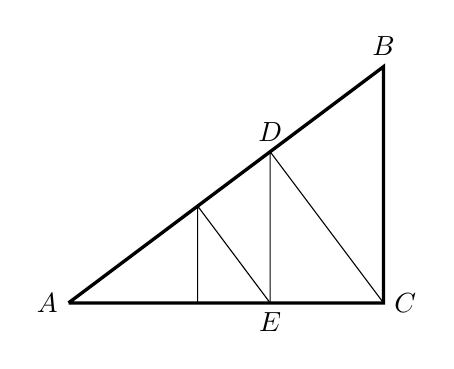
\begin{tikzpicture}[>=latex, scale=1]
\draw[very thick] (0,0)node[left]{$A$}--(4,0)node[right]{$C$}--(4,3)node[above]{$B$}--(0,0);
\draw (4,0)--(2.56,1.92)node[above]{$D$}--(2.56,0)node[below]{$E$};
\draw (2.56,0)--(1.64,1.23)--(1.64,0);
    \end{tikzpicture}
    \caption{}
    \end{minipage}
    \begin{minipage}[t]{0.48\textwidth}
    \centering
    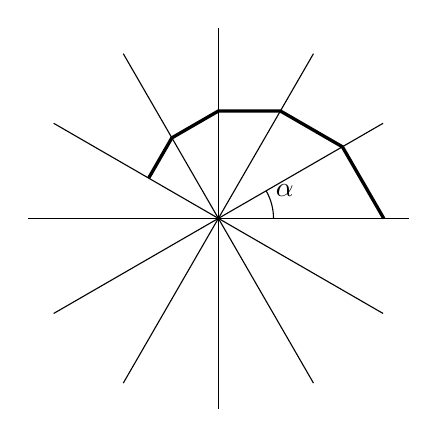
\begin{tikzpicture}[>=latex, scale=.7]
\foreach \x in {0,1,2,...,11}
{
    \draw(0,0)--(30*\x:3.45);
}
\draw[very thick] (3,0)--(30:0.866*3)--(60:0.866*0.866*3)--(90:0.866*0.866*0.866*3)--(120:0.866*0.866*0.866*0.866*3)--(150:0.866*0.866*0.866*0.866*0.866*3);
\draw (1,0) arc (0:30:1)node [right]{$\alpha$};
    \end{tikzpicture}
    \caption{}
    \end{minipage}
    \end{figure}

    \item 直角三角形三边之长分别为3,4,5, 作一圆内切于
    此三角形,再作一圆外切于此圆,并切于三角形的斜边和边长
    为4的直角边,如此继续作下去,则得到一个切圆的序列,
    求这些圆的面积之和。
\end{enumerate}

\section{数列极限存在定理}
前面在引进数列极限的定义时,所考虑的许多数列的极
限都是已经知道的,然后再用数列极限的定义来验证,如果
数列极限的概念仅能给出这样的认识,即一些已知数能够用
另一些已知数的某些数列来逼近,那么我们从极限概念所得
到的东西太少了。但是数列的一个最为重要的应用在于,有
些问题所要确定的数值往往不能用别的方法直接得知或表
示,却能用数列极限方式来表示。例如我们用有理数逼近无
理数,又在上一节用圆内接正多边形的面积来逼近圆面积,
求出$\pi$的数值等,这样的例子就是数列极限重要应用的典型例
子。因此我们构造的数列是否收敛就成为第一位重要问题
了。对于一个数列$\{a_n\}$的极限,事实上应该分成两个层次
来讨论。

\begin{enumerate}
    \item 存在性。即数列$\{a_n\}$是否有极限存在?
    \item 求值问题。假如已经确定了给定数列$\{a_n\}$的极
限存在,我们再设法求它的极限值,其实只要确定了$\{a_n\}$的
极限存在,那么这个极限值就是一个实数,而数列$\{a_n\}$就
是它的逐次逼近的近似数值,要点是去了解数列的性质,总
之求值问题是个比较次要的问题了。 
\end{enumerate}

下面给出一个比较简单的极限存在定理。

\begin{blk}{定理}
    递增有上界的数列$\{a_n\}$极限存在(同样递减,
有下界数列$\{a_n\}$的极限也存在)。
\end{blk}
 
例如:数列$\left\{\frac{n^2-1}{n^2}\right\}$
符合定理的条件,因为
$0,\; \frac{3}{4},\; \frac{8}{9},\; \frac{15}{16},\; \frac{24}{25},\; \ldots$
显然是递增的,同时$a_n=\frac{n^2-1}{n^2}=1-\frac{1}{n^2}<1$, 也就是说,它是有界的,而且容易看出数列
的极限值是1, 事实上
\[\lim_{n\to\infty}\frac{n^2-1}{n^2}=\lim_{n\to\infty}\left(1-\frac{1}{n^2}\right)=1-0=1\]

下面的证明可以说是将二分逼近和实数完备性配合运用
的典型例子,在这儿是初次用到,往后还会遇到相似的配合
用法。其实,只要能基本上理解命题意义和证明大意,就可
以先去学习它的应用,往往用了几次后再回头看第二遍,也
就更加明白了。

\begin{proof}
    一个使得$a_n\le K$恒成立的常数$K$叫做$\{a_n\}$的一个
\textbf{上界}。下面我们将用二分逼近法和完备性来说明$\{a_n\}$的极限
等于它的\textbf{最小上界}(因为$\{a_n\}$是递增的)。

令$A_1=a_1$, $B_1=K$, 由假设$A_1=a_1\le a_n\le K=B_1$, 即所有
$a_n$都在线段$[A_1,B_1]$之内,将线段$[A_1,B_1]$二等分,假如分
点$\frac{1}{2}(A_1+B_1)$
还是一个上界(即$a_n\le \frac{A_1+B_1}{2}$
恒成立),则
取前半段为$[A_2,B_2]$, 不然则取后半段为$[A_2,B_2]$. 这样逐
次二等分,每次当分点$\frac{1}{2}(A_m+B_m)$
是一个上界时,取其前
半段,不然则取其后半段,继续不断地按照上述办法二等分
而选取其半段,就得到满足下列性质的两个夹逼数列$\{A_n\}$
和$\{B_n\}$:

\begin{enumerate}
    \item $A_1\le A_2\le A_3\le \cdots \le A_m\le \cdots \le B_m\le \cdots\le B_3\le B_2\le B_1$, $(B_m-A_m)\to 0$
    \item 所有$B_m$都是数列$\{a_n\}$的上界。
    \item 对于任何$A_m$, 都至少有一个$a_N$使得$A_m<a_N$, 换言
之,线段$[A_m,B_m]$至少包含一个点,比如$a_N$(由$\{a_n\}$的递增
性,所有$n\ge N$也满足$A_m<a_n$)。
\end{enumerate}

因此,由性质1和实数完备性就得到唯一的实数$k$, 
介于一切$A_m$和$B_m$之间,换言之,存在唯一实数$k$使得$\Lim_{m\to\infty}A_m=k=\Lim_{m\to\infty}B_m$

现在让我们来说明$k$也就是$\{a_n\}$的极限!设$\varepsilon$是一个任
给的正数,因为$\Lim_{m\to\infty}A_m=k=\Lim_{m\to\infty}B_m$
所以存在足够大的$M$, 使得(如图7.10)
\begin{figure}[htp]
    \centering
    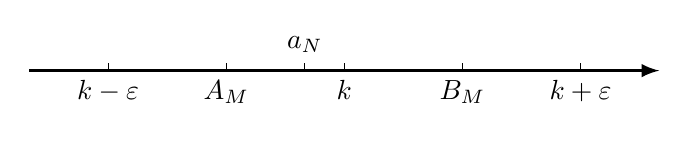
\begin{tikzpicture}[>=latex]
        \draw[very thick,->] (1,0)--(9,0);    
\foreach \x/\xtext in {5/k,2/k-\varepsilon,8/k+\varepsilon,3.5/A_M,6.5/B_M}
{
    \draw (\x,0)node[below]{$\xtext$}--(\x,.1);
}    
\draw (4.5,0)--(4.5,.1)node[above]{$a_N$};
    \end{tikzpicture}

    \caption{}
\end{figure}
\begin{equation}
    k-\varepsilon<A_M\le k\le B_M<k+\varepsilon
\end{equation}
由性质3知道,存在一个够大的$N$, 使得
\begin{equation}
    A_M<a_N    
\end{equation}
由性质2知道,$B_M$是一个上界,即恒有
\begin{equation}
    a_N\le B_M
\end{equation} 
由$\{a_n\}$的递增性,当$n\ge N$时,有
\begin{equation}
    a_N\le a_n
\end{equation} 
综合上述四点,就说明了当$n\ge N$时,有
\[k-\varepsilon<A_M\le a_N\le a_n<B_M<k+\varepsilon\]
亦即$|a_n-k|<\varepsilon$, 这也就说明了
$\Lim_{n\to\infty}a_n=k$。
\end{proof}


\begin{example}
    应用本节存在定理,求$\Lim_{n\to\infty}\frac{r^n}{n!}$。
\end{example}

\begin{solution}
    设$x_n=\frac{r^n}{n!}$,则
\[x_{n+1}=\frac{|r|}{n+1}|x_n|\]
所以只在$n>|r|-1$时,数列$\{|x_n|\}$才是递减的,同时,
由于$|x_n|>0$, 所以它是有下界的,因此数列$\{|x_n|\}$收敛于$\ell$, 在上
面等式两边取极限
\[\Lim_{n\to\infty}|x_{n+1}|=\Lim_{n\to\infty}\frac{|r|}{n+1}\cdot |x_n|\]
即
\[\Lim_{n\to\infty}|x_{x+1}|=\Lim_{n\to\infty}\frac{|r|}{n+1}\cdot \Lim_{n\to\infty}|x_n|\]
因为变量$|x_{n+1}|$和$|x_n|$取同一个数列的数值(除第一个数值
外)。因此有同一个极限$\ell$,即:$\ell=0\cdot \ell$,所以
\[\Lim_{n\to\infty}|x_n|=\ell=0\]
最后有
\[\Lim_{n\to\infty} x_n=\Lim_{n\to\infty} \frac{r^n}{n!} =0\]
\end{solution}

\begin{example}
    求下面数列$\{a_n\}$:
\[\begin{split}
   &  a_1=\sqrt{2},\quad a_2=\sqrt{2+\sqrt{2}},\quad a_3=\sqrt{2+\sqrt{2+\sqrt{2}}},\\
    & \ldots,\quad a_n=\underbrace{\sqrt{2+\sqrt{2+\cdots+\sqrt{2}}}}_{\text{$n$个根号}},\quad\ldots
\end{split} \]
的极限。
\end{example}
   
\begin{solution}
显然,$a_1=\sqrt{2}, a_2=\sqrt{2+a_1},\ldots,
a_n=\sqrt{2+a_{n-1}},\ldots$

$\because\quad 2+\sqrt{2}>2,\qquad \therefore\quad a_2=\sqrt{2+\sqrt{2}}>\sqrt{2}=a_1$

又假设
$a_n>a_{n-1}$成立,
则
$2+a_n>2+a_{n-1}$

$\therefore\quad a_{n+1}=\sqrt{2+a_n}>\sqrt{2+a_{n-1}}=a_n$

因此,对于一切$n\in\mathbb{N}$, 有$a_{n+1}>a_n$, 则此数列是递增的。

$\because\quad \sqrt{2}<2,\qquad \therefore\quad a_1<2,\quad a_2<\sqrt{2+2}=2$

假设$a_{n-1}<2$, 那么,
\[a_n=\sqrt{2+a_{n-1}}<\sqrt{2+2}=2\]
所以对于一切$n\in\mathbb{N}$, 有$a_n<2$。

根据极限存在定理知数列$\{a_n\}$有极限,设它为$x$,于是,
$\Lim_{n\to\infty}a_n=x$。
由于
\[a_n=\sqrt{2+a_{n-1}}\]
两边平方得
\[a^2_n={2+a_{n-1}}\]
取极限有
\[\lim_{n\to\infty}a^2_n =\lim_{n\to\infty}(2+a_{n-1})\]
或者:$x^2=2+x$,解得:
\[x_1=2,\qquad x_2=-1\]
然而因为$a_n>0\quad \Longrightarrow\quad \Lim_{n\to\infty}a_n=x\ge 0$,

$\therefore\quad x_2=-1$不合要求,
因此,
\[\lim_{n\to\infty}a_n=2\]
\end{solution}

由上面的极限存在定理可以引出下面的结论:
\begin{enumerate}
    \item 预先证明极限存在是很重要的,它也给实际计算
这个极限提供了基础。
\item 在极限定义中,要求我们预先猜到$\{a_n\}$的极限值
$A$, 然后再用数列极限定义来验证这个极限$A$是存在的,这
就和前面所说的在数列极限的重要应用中出现的层次有些本
末倒置,本节的极限存在定理就纠正了这种本末倒置的
局面。
\end{enumerate}

\section*{习题7.6}
\addcontentsline{toc}{subsection}{习题7.6}
\begin{enumerate}
    \item 试利用关于单调而有界的数列的极限存在定理检验
    下面数列极限存在性。
\begin{enumerate}
    \item $a_n=1+\frac{1}{1\cdot 2}+\frac{1}{1\cdot 2\cdot 3}+\cdots+\frac{1}{1\cdot 2\cdot 3\cdots (n-1)}$,\quad $n=1,2,3,\ldots$
    \item $a_n=\frac{1}{n+1}+\frac{1}{n+2}+\cdots +\frac{1}{2n}$,\quad $n=1,2,3,\ldots$
    \item $x_n=p_0+\frac{p_1}{10}+\cdots +\frac{p_n}{10^n}$,式中$p_i,\; (i=0,1,2,\ldots)$是非负数,且从$p_1$起不大于9.
\end{enumerate}
\item 已知$a_1=\sqrt{2},\; a_2=\sqrt{2\sqrt{2}},\; a_3=\sqrt{2\sqrt{2\sqrt{2}}},\ldots,a_{n+1}=\sqrt{2a_n},\ldots$, 求 $\Lim_{n\to\infty}a_n$.
\item 设$a_{n+1}=\sqrt{k+a_n}$, 这里$k>0$, $a_1>0$, 求证数列$\{a_n\}$
递增,并以方程$x^2=x+k$的正根为极限。
\item 已知$x_1=1,x_2=1+\frac{x_1}{1+x_1},\ldots,x_n=1+\frac{x_{n-1}}{1+x_{n-1}},\ldots$, 求 $\Lim_{n\to\infty}x_n$.

\item 数列$\{x_n\}$由下面递归方程定义
\[x_1=h,\qquad x_{n+1}=x_n^2+k\]
这里$0<k<\frac{1}{4}$,$h$在方程$x^2-x+k=0$的二根$a,b$之间,
即$a<h<b$。求证:$a<x_{n+1}<x_n<b$, 并求 $\Lim_{n\to\infty}x_n$.

\item 设$0<a_1<b_1$是两个给定正数,令
\[\begin{split}
    a_2&=\sqrt{a_1b_1},\qquad b_2=\frac{1}{2}(a_1+b_1),\quad (a_2<b_2)\\
    a_3&=\sqrt{a_2b_2},\qquad b_3=\frac{1}{2}(a_2+ b_2),\quad (a_3<b_3)\\
\cdots &\cdots\cdots\cdots\cdots\\
    a_{n+1}&=\sqrt{a_nb_n},\qquad b_{n+1}=\frac{1}{2}(a_n+b_n),\quad (a_{n+1}<b_{n+1})\\
\end{split}\]
求证:
\begin{enumerate}
    \item $\{a_n\}$递增和$\{b_n\}$递减;
    \item $\{a_n\}$和$\{b_n\}$的极限相同。
\end{enumerate}
\end{enumerate}